\documentclass[a4paper]{article}
\title{Workshop on Public Key Infrastructure \\
and \\
Red Hat Certificate System}
\author{\underline{Asha Akkiangady, Huzaifa Sidhpurwala, Niranjan Mallapadi}}
\date{}
\usepackage{color}
\usepackage{xcolor}
\usepackage{graphics}
\usepackage{graphicx,subfig}
\usepackage{listings}
\usepackage{color}
\usepackage{enumitem}
\usepackage{float}
\usepackage{url}
\usepackage{hyperref}
\hypersetup{
    colorlinks=true, 
    linktoc=all,     
    linkcolor=blue,
}
\bibliographystyle{plain}
\definecolor{dkgreen}{rgb}{0,0.6,0}
\definecolor{gray}{rgb}{0.5,0.5,0.5}
\definecolor{mauve}{rgb}{0.58,0,0.82}
\lstset{frame=tb,
  aboveskip=3mm,
  belowskip=3mm,
  showstringspaces=false,
  columns=flexible,
  basicstyle={\small\ttfamily},
  numbers=none,
  commentstyle=\color{dkgreen},
  breaklines=true,
  breakatwhitespace=true,
  tabsize=3
}
\lstdefinestyle{BashInputStyle}{
    language=bash,
    basicstyle={\small\ttfamily},
    showstringspaces=false,
    showspaces=false,
    numberstyle=\tiny,
    numbersep=1pt,
    frame=tb,
    columns=fullflexible,
    backgroundcolor=\color{red!5}
}
\begin{document}
\maketitle
\tableofcontents
\section{Introduction to Public Key Cryptography}
Before we start discussing about public key cryptography, we will in general discuss about how systems communicate
and what are the various threat models that are associated with the communication medium and what are the tools to 
overcome them.~\cite{eric}

\textbf{Example1:}
The most common protocol used to communicate between 2 systems is TCP/IP. TCP/IP allows information to be sent 
from one system to another system directly or through many intermediate systems.~\cite{eric}

Below are some of the threat models associated with TCP/IP:
\begin{itemize}
    \item \textbf{Eavesdropping:}
        
        Information remains intact, but it's privacy is compromised. For example: someone could retrieve the credit card number, 
          record a sensitive conversation or intercept a classified information.
    \item \textbf{Tampering:}

        Information in transit is changed or replaced and then sent to the recipient. For example: Some one could alter an order of goods or change a persons resume.
    \item \textbf{Impersonation:}

        Information passes to a person who poses as intended recipient. Impersonation can take 2 forms:
    \begin{itemize}
        \item \textbf{Spoofing:}

            A person can pretend to be someone else, For example, a person can pretend to have email address \textit{joe@example.net}, 
            or computer can identify itself as a site called www.example.net, when it is not. This type of impersonation is called spoofing.
        \item \textbf{Misrepresentation:}

            A person or organization can misrepresent itself, For example, suppose the site \textit{www.example.net} pretends to be a 
            furniture store when it's just a site which accepts payments but never sends any goods.
    \end{itemize}
\end{itemize}
\textbf{Example2:}
Consider Alice , Bob and attacker are the parties , where alice and bob want to communicate 
to each other and Attacker is a threat to the communication.~\cite{eric}

\begin{itemize}
    \item Alice can send a postcard to bob to communicate, but this method is very weak as any random eavesdropper could read the postcard.
    \item Alice could write a letter and put in an envelope and send it to bob, but the attacker could open the envelope and read the letter, 
        both confidentiality and integrity of the message is lost.
    \item Alice could seal the envelope with wax , but this method too is inefficient as Attacker could read the letter and seal it as it is 
        without bob knowing that it was read by attacker
    \item Alice could write a letter and put it in a safe which has 2 keys and send one key before to Bob , and send the safe across to bob, 
        this ensures confidentiality, integrity but practically this is not implementable. Considering the number of 
        messages that has to be transferred , it's impractical to implement the mail safe method.
\end{itemize}

To mitigate above threat models, we will look in to cryptology as one of the tools of the trade. 

\textbf{Cryptology:} Cryptology is the theory of designing the various algorithms we use to provide security

\textbf{Cryptography:} Cryptography is the study of using these algorithms to secure systems and protocols.
\subsection{Encryption}
An encryption algorithm takes some data(called plaintext) and converts it to cipher-text under control of a key. 
cipher text contains random data which makes no sense without the key.  

A key is a short random string (8-24 bytes): 

\begin{picture}(10,10)(10,10)
    \put(40,1){\framebox(55,8){Plain Text}} 
    \put(102,10){\tiny Encryption}
    \put(102,4){\vector(1,0){30}}
    \put(140,1){\framebox(55,8){Cipher Text}} 
    \put(200,10){\tiny Decryption}
    \put(200,4){\vector(1,0){30}}
    \put(240,1){\framebox(55,8){Plain Text}} 
\end{picture}
\linebreak

When a message is encrypted and received , we cannot say if it's not tampered with. An encryption is strong when 
it can determine the number of possible keys. The attacker tries each key one at a time until he finds a key that 
produces a plausible decryption. The security of the algorithm should solely depend on the secrecy of the key. 
The algorithm should not need to be secret.

If the attacker knows the plaintext corresponding to the ciphertext it's called \textit{``known plaintext attack''} .

An attack where attacker doesn't know the plaintext , it's called \textit{``ciphertext-only attack''}.
\textit{Ex:} If the attacker knows that plaintext is ASCII , so any decryption which uses non-ascii characters must be using the wrong key.
\subsubsection{Symmetric Encryption}
When Sender and recipient share the same key(which must be kept secret) is referred to as \textit{Symmetric Key Cryptograph} or also
referred to as \textit{Secret Key Cryptography} as opposed to \textit{Public Key Cryptography}~\cite{eric}.
\begin{figure}[h]
    \centering
    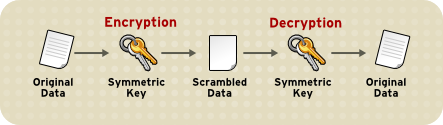
\includegraphics[width=50mm]{symmetric.png}
    \caption{Symmetric Encryption ~\cite{RedHat:Symmetric}}
\end{figure}
\subsubsection{Assymetric Encryption}
\begin{itemize}
    \item First started in stanford university by Whitfield Diffie and Martin Hellman
    \item The most commonly used implementation of PKC are based on algorithm based on algorithm patented by RSA data security.
    \item Each public key is published \& private key is kept secret. Data encrypted with public key can be decrypted only with private key.
    \item In general, to send encrypted data to someone, we encrypt with public key \& the person receiving the 
        encrypted data decrypts with private key
    \item Compared to symmetric key encryption, public key encryption requires more computation \& therefore not always appropriate for large amounts of data
    \item It is possible to use public-key encryption to send a symmetric key, which can then be used to encrypt additional data.
        \begin{figure}[h]
            \centering
            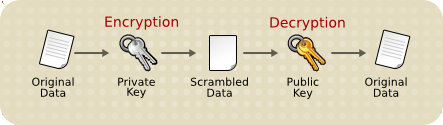
\includegraphics[width=80mm]{assymetric.png}
            \caption{Assymetric Encryption}
        \end{figure}
    \item Reverse of the above figure also happens i.e. encrypt with private key and decrypt with public-key. But not useful for sensitive information
        \begin{figure}[h]
        \centering
        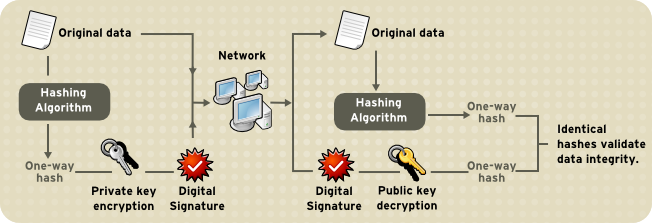
\includegraphics[width=80mm]{digitalsignature.png}
        \caption{Digital Signature ~\cite{RedHat:CSoverview}} 
        \end{figure}
    \item There's a problem with the above method, how would the parties get each other's public-key ? 
        If we send the keys through electronically, then the attacker an tamper, while they are in transit to the receiver.
    \item When the 2 parties want to communicate, the attacker can intercept the keys \& instead send his own key to each other, 
        thus each party encrypts to him and \& he re-encrypts it to the real recipient. 
        This is called \textit{man-in-the-middle attack}
\end{itemize}
\subsection{Message Digest}
A message digest is simply a function that takes as an input an arbitrary message and outputs a fixed length string 
which is characteristic of the message. The important property here is irreversibility.  
It's extremely difficult to compute a message from the given digest. 
Property of the message digest: 
\begin{itemize}
    \item For a digest to be secure, it must be difficult to generate any of the message that digests to the same value. 
        You have to search a message space of proportional size of the digest in order to find a matching message text
    \item It should be difficult to produce 2 messages M and M' such that they have the same digest. 
        This property is called collision-resistance. It turns out that the strength of any message digest 
        against finding collision is only half the size of the digest., so a 128-bit digest is only 64 bits strong against collisions.
\end{itemize}
\subsubsection{Message Authentication Code}
Consider \textit{Alice} and \textit{Bob} share a key and Alice wants to send a message to \textit{Bob}. The message can be encrypted, 
and send it across to \textit{Bob}, but we are not sure that the encrypted message would be tampered and also not sure 
if \textit{Alice} was the one who sent the encrypted message.  So we use a new tool called \textit{MAC} . \textit{MAC} is a digest algorithm,
but with a key, So the MAC is dependent on both the key and the message being MACed ~\cite{eric}.
\subsection{Algorithms}
\begin{itemize}
    \item \textbf{RSA ~\cite{eric}}
        \begin{itemize}
            \item RSA is the public-key algorithm widely used in Public-key Cryptography
            \item Invented by Ron-Rivest, Adi Shamir and Len Adelman (RSA). Each user has a public-key and a private-key
            \item The public-key can be freely distributed and the private-key must be kept secret.
            \item Brief Explanation:
                \begin{itemize}
                    \item Generate 2 prime numbers (3, 17), call them p and q
                    \item n = modulus(p * q)
                    \item p and q are kept secret
                    \item Difficulty is in factoring m, so that we get p and q
                    \item Take another number "e" which is called public exponent, which is a prime
                        number , it's usually small prime numers {3, 17 or 65537}
                    \item Compute d = $e^{-1}mod((p-1)(q-1))$
                    \item Public Key = (e, n)
                    \item Private Key = (d, n)
                    \item Message M is encrypted with public key and decrypted with private key
                    \item RSA assumes that M is a number,  So we need a convention to convert strings in to numbers.
                \end{itemize}
        \end{itemize}
    \item \textbf{DSA ~\cite{eric}}
        \begin{itemize}
            \item National Institute of standards and technology (NIST) published the Digital signature
                algorithm in the Digital signature standard.  
            \item Compared to RSA where it can be used for both encryption and digital signature
            \item In DSA the signature generation is faster than signature verification
        \end{itemize}
    \item \textbf{RC4}
        \begin{itemize}
            \item RC4 is a stream cipher.
            \item Assume we have a function (f) which produces 1 byte of data. 
                This output is called keystream (ks)
            \item The function (f) takes a encryption key as an input to generate keystream
            \item Without the key we can't predict keystream
            \item So combine each byte with one byte of plain text which is our cipher-text
            \item C[i] denotes the ith unit of ciphertext 
            \item where a unit refers a 1 byte of data.
            \item ks[i] refers the ith unit of keystream
            \item M[i] refers to the ith unit of the message.
            \item C[i] = ks[i] xor M[i]
            \item m[i] = ks[i] xor C[i] 
            \item Disadvantages:
                \begin{itemize}
                    \item Assume we have used the same key to encrypt the Messages M and M' 
                    \item If the attacker learns M and can compute ks by simply computing M xor C.
                    \item Once the attacker knows KS he can generate M'
                \end{itemize}
            \item RC4 was designed by Ron Rivest . RC4 is a variable key length cipher , with key can be
                anywhere between 8 to 2048 bytes long
            \item SSL/TLS protocol use RC4 with 128-bit (16 bytes) key length
            \item RC4 is extremely fast. 
        \end{itemize}
    \item \textbf{Block Ciphers}~\cite{eric}
        \begin{itemize}
            \item \textbf{DES}
                \begin{itemize}
                    \item The data to be encrypted is processed in blocks of bytes  (8 or 16).
                    \item Each possible plain text block corresponds to a row in the table
                    \item So to encrypt a block you find a column corresponding to the key, 
                        run down the table to find the row corresponding to the block you want 
                        to encrypt. 
                    \item If the data is huge, it's very difficult to manage, 
                        so we define a function that does the computation
                    \item The idea is to simulate a random table
                    \item  we have a key(k), and a data block .  and we define 2 function E for encryption ,and
                        D for decryption
                    \item C=E(K,M)
                    \item M=D(k,c) 
                    \item When we have large messages , we do in Electronic code book mode. 
                        \begin{itemize}
                            \item Break the message up to block sized-chunks.
                            \item individually encrypt it using encryption algorithm 
                            \item C[i]=E(k,M[i])
                            \item M[i]=D(K,C[i]) 
                        \end{itemize}
                    \item DES was desinged by IBM , it's  patented but freely available
                    \item DES is a 64 block cipher with 56-bit key . The data is encrypted in blocks of 8 bytes and a key space of 56 bits.
                    \item DES is used with public-key techniques. 
                    \item Disadvantages:
                        \begin{itemize}
                            \item if M[i] and M[j] are same, then we get the same C[j] and C[k]. Attacker can get the pattern
                            \item Cipher block chaining mode, The encryption of each plain text block M[i] depends on 
                                cipher text of previous block C[i-1].
                            \item That can be accomplished by XORing previous Cipher text block C[i-1]] Xor M[i] before encryption
                         \end{itemize}
                    \end{itemize}
                \item \textbf{3DES}~\cite{eric}
                \begin{itemize}
                    \item Run the DES algorithm 3 times.
                    \item It's  used in Encrypt-Decrypt-Encrypt (EDE mode).
                    \item Message is encrypted with key-1, Decrypted with Key-2 and Encrypted with key-3.  
                    \item 3DES is 3 times slower than DES.
                \end{itemize}
            \item \textbf{RC2}~\cite{eric}
                \begin{itemize}
                    \item RC2 is a block cipher invented by Ron Rivest,
                    \item RC2 is a variable-length cipher , with variable length key.  It uses 64 bit block size.
                \end{itemize}
            \item \textbf{AES}~\cite{eric}
                \begin{itemize}
                    \item Advanced Encryption Standard uses a minimum of 128 bits and 3 key lengths, 128. 192 and 256 bits
                \end{itemize}
        \end{itemize}
    \item \textbf{Digest Algorithms}~\cite{eric}
        \begin{itemize}
            \item The two most popular Digest Algorithms are MD5, which was designed by Ron Rivest and SHA-1 by NIST.
            \item MD5 and SHA share a common ancestor MD4 also designed by Ron Rivest
        \end{itemize}
\end{itemize}
\subsection{Protocols}
\subsubsection{SSL}
    \begin{itemize}
        \item Secure Socket Layer (SSL) is a protocol that provides a secure channel between machines
        \item It has facilities for protecting data in transit and identifying machine with which it is begin communicated
        \item Protocol is transparent , so it can be run on any protocol. 
        \item SSL has gone through many versions and currently is culminating with the adoption by IETF as Transport Layer Security
        \item SSL was originally designed for world wide web , but also was intended as a unifying solution to all the other communications (web, mail, news traffic)
        \item The current version of SSL is tlsv2 which fixes a lot of security problems
        \item \textbf{Overview of SSL Protocol}
            \begin{itemize}
                \item Primary goal of SSL is to provide privacy and reliability between 2 communicating applications
                \item The protocol is composed of 2 layers : \textbf{Handshake protocol} and \textbf{record protocol}
                \item \underline{In brief Handshake protocol provides}
                    \begin{itemize}
                        \item allows server \& client to authenticate to each other
                        \item Negotiate encryption algorithm or Cryptography keys. 
                    \end{itemize}
                \item \underline{Record protocol provides:}
                    \begin{itemize}
                        \item Confidentiality
                        \item Authenticity
                        \item replay protection
                    \end{itemize}
            \end{itemize}
        \item \textbf{Handshake Protocol}
            \begin{itemize}
                \item Client sends a list of algorithms it's willing to support along with a random number
                    used as input to a key generation proces
                \item Server chooses out of that list and sends it back along with a certificate
                    containing servers public-key. 
                \item certificate also provides the server's identity for authentication purpose and the 
                    server supplies a random number which is used as a part of key generation process
                \item Client verifies the servers certificate and extracts the server's public-key
                    from the certificate
                \item Client then generates a random secret called \textit{pre\_master\_secret} and encrypts this 
                    with  server's public-key
                \item Client sends this encrypted \textit{pre\_master\_secret} to the server 
                \item Client and the Server independently compute the encryption and MAC keys from 
                    \textit{the pre\_master\_secret} and client and server's random values
                \item Client sends a MAC of all the handshake messages to the server
                \item The server sends a MAC of all the handshake messages to the client
                \item \begin{figure}[ht!]
                        \centering
                        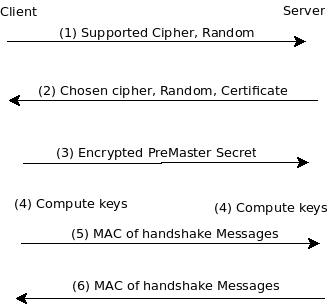
\includegraphics[width=40mm]{sslhandshake1.png}
                        \caption{SSL Handshake}
                      \end{figure}
                \item Step:1 corresponds to single SSL Handshake message, Client Hello
                \item Step:2 corresponds to SSL Handshake messages
                    \begin{itemize}
                        \item First is a ServerHello { Algorithm preference, Certificate }
                        \item Send ServerHelloDone
                    \end{itemize}
                \item Step3 correponds to ClientKeyExchange
                \item Step 5 and 6 correspond to the finished message. The Finished message is the first
                    message that's the protected using Just-Negotiated algorithms.
                \item To protect the handshake from tampering, the content of the message is MAC of 
                    all the previous handshake messages
                \item \begin{figure}[ht!]
                        \centering
                        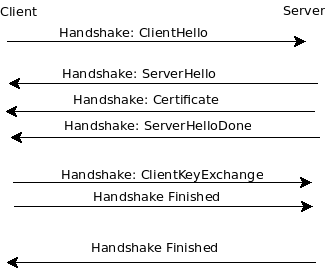
\includegraphics[width=40mm]{sslhandshake2.png}
                        \caption{SSL Handshake}
                      \end{figure}
                \item \textbf{Resuming Session}
                    \begin{itemize}
                        \item client sends a clientHello with a Session-ID of the session to be resumed.
                        \item server check it's session cache for a match
                        \item If the match is found \& the server is willing to re-establish the connection under specified
                            session state , it will send a ServerHello with same session-ID
                        \item At this point both client and server must send change Cipher spec messages \& proceed
                            directly to finished messages 
                        \item There is no exchange of certificates here.
                        \item Once the re-establishment is complete the client \& server may begin exchange of application data
                        \item If the Session-ID match is not found the server generates a new session-ID \& the client and
                            Server have to perform a full handshake
                    \end{itemize}
           \end{itemize}
        \item \textbf{SSL Record Protcol}
            \begin{itemize}
                \item The actual data transfer is accomplished by SSL Record Protocol
                \item Record Protocol works by breaking up the data stream to be transmitted in to a series of
                    fragments, each of which is independently protected and transmitted.
                \item On the receiving end , each record is independently decrypted and verified.
                \item Before transmission , a  MAC is computed on each record , This MAC is transferred along with the record
                \item The concatenated data and MAC are encrypted to form encrypted Payload. We attach a header to 
                    that encrypted payload which we refer to as a record
                \item \begin{figure}[ht!]
                        \centering
                        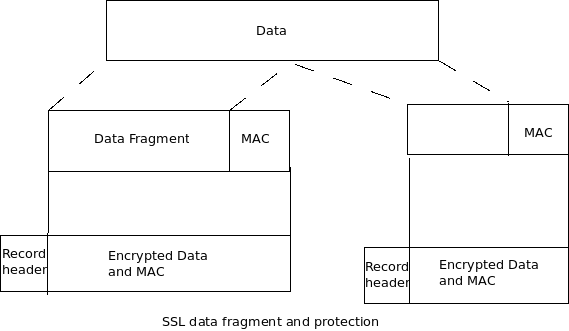
\includegraphics[width=50mm]{ssldatafrag.png}
                        \caption{ssl data fragment and protection ~\cite{eric}}
                      \end{figure}
                \item The record header provides the information for the other end to interpret the record. It contains:
                    \begin{itemize}
                        \item Content Type (Application data, alert messages, handshake message, change cipher spec)
                        \item length  (how many bytes to read off wire)
                        \item SSL Version
                    \end{itemize}
                \item The \textit{change\_cipher\_spec} message indicates a change in encryption and authentication of records
                \item Once the handshake is completed a new set of keys is negotiated, \textit{change\_cipher\_spec} record is 
                    sent to indicate that those keys will now be used.
                    \begin{figure}[H]
                        \centering
                        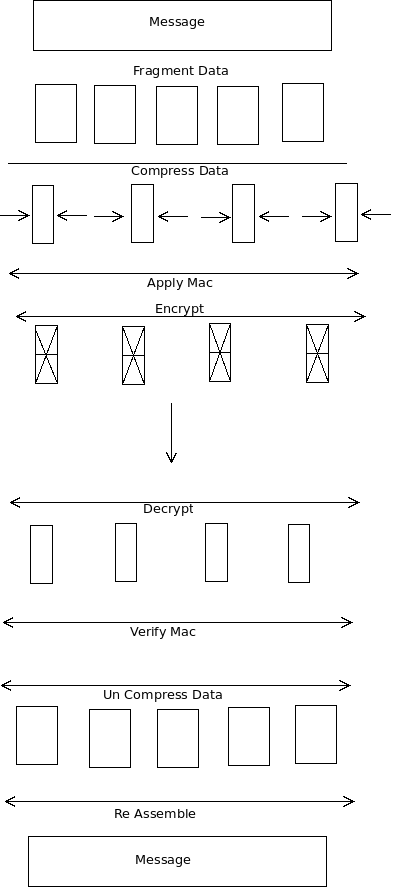
\includegraphics[width=30mm]{ssl-overview.png}
                        \caption{SSL Overview}
                    \end{figure}
            \end{itemize}
    \end{itemize}
\section{Introduction to Public Key Infrastructure}
Below is a simplified architectural model of Public Key Infrastructure using X.509 (PKIX) Specifications
\begin{figure}[ht!]
    \centering
    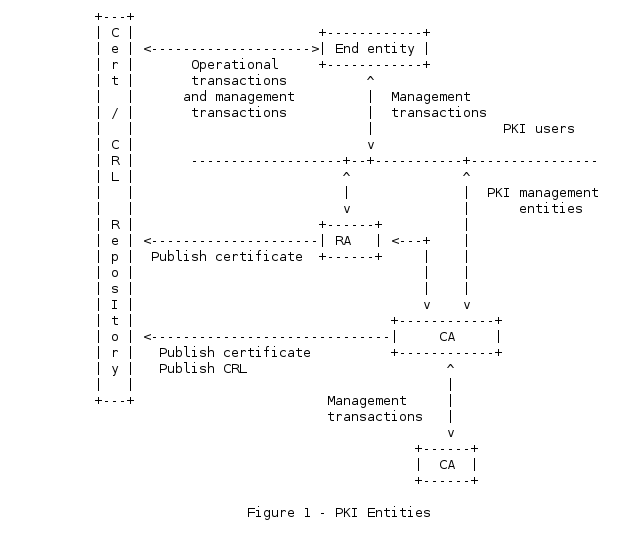
\includegraphics[width=70mm]{pki-architectural-model.png}
    \caption{PKI Architectural Model ~\cite{5280}}
\end{figure}
\subsection{Common Terms used in PKI}
\begin{itemize}
    \item \underline{End Entiy}: User of the PKI certificates and/or end user system that is the subject of a certificate
    \item \underline{CA}: Certificate Authority
    \item \underline{RA}: Registration Authority, Optional System to which CA delegates certain management functions
    \item \underline{CRL issuers}: A system that generates CRL
    \item \underline{repository}: a system or collection of distributed systems that stores certificates and CRLs and services as a means of distributing these certificates and CRLs to end entities
\end{itemize}
\subsection{Detailed look on certificate/CRL}
    \subsubsection {Certificates}
        \begin{itemize}
            \item Certificates are data structures that bind public key values to the subject. This binding is asserted by a trusted Certificate Authority.
            \item X.509 defines the standard certificate format and v3 is the latest version.
            \item Internet Privacy Enhanced Mail(PEM) RFC 1421 and 1422 also include specifications for PKI based on X.509 certs. 
            \item Types of Certificates:
                \begin{itemize}
                    \item End-Entity
                    \item CA
                \end{itemize}
            \item RFC 1422 defines hierarchial structure  of CA's and there are three types of PEM CA
                \begin{itemize}
                    \item IPRA: Internet Policy Registration Authority , acts as Root of Certificate authority. IPRA operates under Internet Society Organization
                    \item PCA: Policy Certificae Authority ,(Verisign, Digicert, etc) signed by IPRA
                    \item CA: Certificate Authorities signed by PCA (Organizational CA's)
                \end{itemize}
            \item Policies used by CA:
                \begin{itemize}
                    \item IPRA certifies only PCA and not CA's or users cert
                    \item IPRA will make sure that the DN of the PCA is unique and will not certificate PCA's with similar DN
                    \item Certificates should not be issued to distinct entities under the same distinguished Name. 
                    \item IPRA should not certifiy two PCA's with same DN
                    \item PCA's should not certify two CA's with same DN
                    \item CA's are expected to sign certificates only if the subject DN in the
                        certificates is subordinate to the issuer CA DN.
                \end{itemize}
            \item Types of Certificate Authorities
                \begin{itemize}
                    \item Cross-Certs: Where Issuer and Subject are different
                    \item Self-Issue: Where Issuer and Subject are same
                        \begin{itemize}
                            \item Self-Signed: Where key bound in to the certificate is same as the key used to sgin the certificate
                        \end{itemize}
                \end{itemize}
        \end{itemize}
    \subsubsection{Basic Certificate Fields}
        \begin{itemize}
            \item Version:
                \begin{itemize}
                    \item Describes the version of encoded certificate.
                    \item if extensions are used: \textbf{0x2(3)}
                    \item if extensions are not used but UniqueIdentifier is used: \textbf{0x1(2)}
                    \item if only basic fields are there: \textbf{0x0(1)}
                \end{itemize}
                \begin{itemize}
                    \item Values: \textbf{0x2(3), 0x1(2), 0x0(1)}
                \end{itemize}
            \item Serial Number:
                \begin{itemize}
                    \item Positive integer assigned by CA to each certificate
                    \item It must be unique for each Certificate given by CA
                    \item Can contain long integers (up to 20 Octets)
                \end{itemize}
                \begin{itemize}
                    \item Values: Integers: 
                    \begin{itemize}
                        \item \textbf{16694152257348400000}
                        \item \textbf{0xe7ad8b07558a1727}
                        \item \textbf{cd:ba:7f:56:f0:df:e4:bc:54:fe:22:ac:b3:72:aa:55}
                    \end{itemize}
                \end{itemize}
            \item Signature:
                \begin{itemize}
                    \item Algorithm used by \textbf{CA} to sign the certificate
                    \item Value:
                        \begin{itemize}
                            \item \textbf{md2WithRSAEncryption}
                            \item \textbf{sha1WithRSAEncryption}
                        \end{itemize}
                \end{itemize}
            \item Issuer:
                \begin{itemize}
                    \item Identifies the entity that has signed and issued the certificate
                    \item \textbf{MUST} contain non-empty Distinguished Names
                    \item Names should confirm to X.501 standard
                    \item Generally contains Country, Organization, Common name, SerialNumber,
                        province, State, title, Surname, Generation Qualifier(Jr, Sr).
                    \item Values:
                    \begin{itemize}
                        \item \textbf{C=US, O=VeriSign, Inc., OU=Class 1 Public Primary Certification Authority}
                        \item \textbf{C=DE, ST=Bayern, L=Muenchen, O=Whatever it is, CN=IO::Socket::SSL Demo CA}
                        \item \textbf{C=US, O=VeriSign, Inc., OU=Class 1 Public Primary Certification Authority}
                    \end{itemize}
                \end{itemize}
            \item Validity:
                \begin{itemize}
                    \item The time interval during which the CA warrants that it will maintain status of the certificate
                    \item Consists sequence of 2 dates
                        \begin{itemize}
                            \item Date on which certificate validity begins
                            \item Date on which certificate validity ends
                        \end{itemize}
                    \item Validity period of a certificate is period from notBefore to notAfter(inclusive)
                    \item Values:
                        \begin{itemize}
                            \item \textbf{Not Before: Jan 29 00:00:00 1996 GMT}
                            \item \textbf{Not After : Aug  1 23:59:59 2028 GMT}
                            \item Special Note:
                                \begin{itemize}
                                    \item Devices are given certificates where there is no expiration date
                                    \item Value:
                                    \item Certificate is to be used for entire lifetime of the device \textbf{ Not After: 99991231235959Z.(represented in Generalized Time)}
                                \end{itemize}
                        \end{itemize}
                    \end{itemize}
            \item Subject:
                \begin{itemize}
                    \item Identifies the entry associated with public key stored in the subject public key field 
                    \item If the subject is CA then it should be populated with same data as issuer 
                    \item Names should confirm to X.501
                    \item Values:
                        \begin{itemize}
                            \item \textbf{C=US, ST=North Carolina, O=Fedora Project, OU=Fedora User Cert, CN=mrniranjan/emailAddress=niranjan@ashoo.in}
                        \end{itemize}
                \end{itemize}
            \item Subject Public key Info:
                \begin{itemize}
                    \item This field is used to carry public key and identify the algorithm with which the key is used (RSA, DSA)
                    \item Supported Cryptographic Algorithms:
                        \begin{itemize}
                            \item \textbf{Rivest-Shamir-Adelman (RSA)}
                            \item \textbf{Digital Signature Algorithm (DSA)}
                            \item \textbf{Diffie-Hellman (DH)}
                            \item \textbf{Elliptic Curve Digital Signature Algorithm (ECDSA)}
                            \item \textbf{Key Encryption Algorithm (KEA)}
                            \item \textbf{Elliptic Curve Diffie-Hellman (ECDH)}
                        \end{itemize}
                \end{itemize}
            \end{itemize}
    \subsubsection{Extensions}
        \begin{itemize}
            \item This field only appears in v3 Certs
            \item This contains sequence of one or more Certificate Extensions 
            \item Extensions provides method for associating additional attributes with public keys
            \item Managing relationship between CA's
            \item Can carry private extensions to carry information unique to their community
            \item Each Extension is either Critical / Non Critical
            \item Each Extension includes OID and ASN.1 DER  (OCTET)
                \begin{itemize}
                    \item Example: DE:65:01:16:19:2E:51:E0:9A:51:1A:37:50:94:7D:39:29:2A:42:2C
                \end{itemize}
            \item There cannot be duplicates of Extensions
            \item Default CRITICAL value is false
            \item If the Certificate is CA , then they should have below Extensions
                \begin{itemize}
                    \item Basic Key Identifier
                    \item Authoritative key Identifier
                    \item Basic Constraints
                \end{itemize}
        \end{itemize}
        \begin{itemize}
            \item \textbf{Authority Key Identifier:}
                \begin{itemize}
                    \item Provides a means of identifying the public key corresponding to the private key used to sign the certificate
                    \item This is required if the issuer has multiple signing keys 
                    \item If the CA certificate is self signed Authority key identifier is skipped
                    \item Authority key Identifier helps in identifying the issuer certificate. 
                    \item Values:
                        \begin{itemize}
                            \item \textbf{keyid:48:E6:68:F9:2B:D2:B2:95:D7:47:D8:23:20:10:4F:33:98:90:9F:D4}
                        \end{itemize}
                \end{itemize}
            \item \textbf{Subject Key Identifier:}
                \begin{itemize}
                    \item Provides a means of identifying certificates that contain a particular public key
                    \item This extension is must for CA certificates
                    \item The value placed in this is same as Authority Key Identifier
                    \item For End-entity Certificates, this extension provides a means for identifying certificates containing particular key used in application
                    \item Value:
                        \begin{itemize}
                            \item \textbf{48:E6:68:F9:2B:D2:B2:95:D7:47:D8:23:20:10:4F:33:98:90:9F:D4}
                        \end{itemize}
                \end{itemize}
            \item \textbf{Key Usage:}
                \begin{itemize}
                    \item Defines the purpose of the key contained in the certificate 
                    \item This extension is used to restrict the usage of the key to be used for purpose 
                        other than what is defined in Key Usage
                    \begin{itemize}
                        \item \textbf{digitalSignature}
                            \begin{itemize}
                                \item Public key should be used only to verify signatures on objects other than Public key certificates/CRL
                            \end{itemize}
                        \item \textbf{nonRepudiation/contentCommitment}
                            \begin{itemize}
                                \item subject Public key is used to verify digital signatures other than signatures on public key(CRL)
                                \item used to provide nonRepudiation Service that protects against signing entity falsely denying any public action
                            \end{itemize}
                        \item \textbf{keyEncipherment}
                            \begin{itemize}
                                \item Public key is used for enciphering private key or secret keys , 
                                \item Is used for encrypting symmetric content-decryption key or an assymetric private key
                            \end{itemize}
                        \item \textbf{dataEncipherment}
                            \begin{itemize}
                                \item is used for enciphering the raw data without the use any cipher  (very rarely used)
                            \end{itemize}
                        \item \textbf{keyAgreement}
                            \begin{itemize}
                                \item is used for key Agreement, 
                                \item when used Deffie-Hellman key is to be used for key management
                            \end{itemize}
                        \item \textbf{keyCertSign}
                            \begin{itemize}
                                \item Public key is used for verifying the signatures on public keys , if this is true then 
                            \end{itemize}
                        \item \textbf{cRLSign}
                            \begin{itemize}
                                \item when the subject public key is used for verifying signatures of CRL 
                            \end{itemize}
                        \item \textbf{encipherOnly}
                            \begin{itemize}
                                \item subject's public key may be used only for enciphering data while performing key agreement
                            \end{itemize}
                        \item \textbf{decipherOnly}
                            \begin{itemize}
                                \item subject's public key may be used only for deciphering data while performing key agreement
                            \end{itemize}
                        \item Important Note:
                            \begin{itemize}
                                \item \begin{figure}[ht!]
                                    \centering
                                    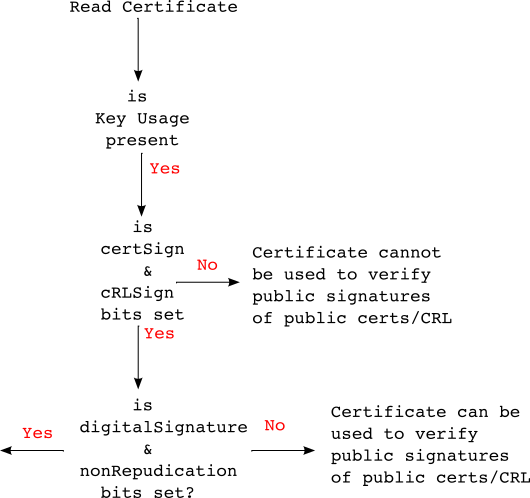
\includegraphics[width=70mm]{KeyUsage1.png}
                                    \caption{Key Usage restrictions}
                                \end{figure}
                            \end{itemize}
                    \end{itemize}
                \end{itemize}
            \item \textbf{Certificate Policies}
                \begin{itemize}
                    \item Contains sequence of one or more policy information terms each of which consits of
                        OID, optional Queries
                    \item OID Should not appear more than once
                    \item for End-entity policy information terms indicate the policy under which the certificate
                        has been issued and purposes for which the certificate must be used
                    \item For CA the policy limits the policies for certificate paths that include this certificate
                    \item if CA does not want to limit the set of policies for certification paths then it may assert
                        \textbf{anyPolicy} with value \textbf{2.5.29.32.0}
                    \item Policy Qualifiers:
                        \begin{itemize}
                            \item CPSNotice: Points URL to \textit{certificate practice statement} document that describes
                                the policy under which the subject was issued
                            \item userNotice: text that describes the policy(not more than 200 characters)
                        \end{itemize}
                \end{itemize}
            \item \textbf{Policy Mappings}
                \begin{itemize}
                    \item This extension is used by CA certificates 
                    \item Lists one or more pairs of OID, which indicate that the corresponding policies 
                        of one CA are equivalent to policies of another CA [used in context of Cross pair certificates]
                    \item \textbf{OID: 2.5.29.33}
                \end{itemize}
            \item \textbf{Subject Alternative Name}
                \begin{itemize}
                    \item Allows alternate names to be bound to subject of the certificate. 
                    \item The names specified in subjectAltName may be included in addition to
                        or in place of the identity in the subject field of the certificate
                    \item Defined subject names used:
                        \begin{itemize}
                            \item rfc822Name:       IA5String
                            \item otherName:        OtherName
                            \item dNSName:          IA5String
                            \item directoryName:    Name
                            \item URI:              IA5string
                            \item iPAddress:        OCTET String
                            \item UniformResourceIdentifier: IA5String
                        \end{itemize}
                \end{itemize}
            \item \textbf{Issuer Alternative Name}
                \begin{itemize}
                    \item Allows alternate names to be bound to certificate issuer
                    \item Issuer alternative names are not processed as part of certification path validation
                    \item Issuer Alternative name extension when present should be non-critical
                \end{itemize}
            \item \textbf{Subject Directory Attributes}
                \begin{itemize}
                    \item This extension is used to convey identification attributes of the subject
                    \item Value:
                        \begin{itemize}
                            \item nationality of the subject
                        \end{itemize}
                \end{itemize}
            \item \textbf{Basic Constraints}
                \begin{itemize}
                    \item This extension identifies whether the subject of the certificate is CA ?
                    \item It also identifies Maximum depth of valid certification paths that include this certificate
                    \item Values:
                        \begin{itemize}
                            \item cA: (boolean): indicates whether certificate is CA cert
                            \item pathLenConstraint: applicable if cA boolean is true. if prsent asserts keyCertSign bit. 
                            \item It gives maximum number of non-self-issued intermediate Certificates that may follows this certificate in a valid certification path. The last cert is End-entity certificate
                            \item Ex: PathLength is 2:
                                \begin{itemize}
                                    \item RootCA - EE Cert
                                    \item RootCA - subca1-EE Cert
                                    \item RootCA - subca1-subca2-EE Cert
                                    \item RootCA - subca1-subca2-subca3-EE Cert
                                \end{itemize}
                        \end{itemize}
                \end{itemize}
            \item \textbf{Name Constraints}
                \begin{itemize}
                    \item Used only in CA certificate
                    \item Specifies name space within which all subject names in 
                        subsequent certificates ina certification path MUST be located.
                    \item Restrictions apply to Subject Dishtinguished Name and 
                        subject alternative names.
                    \item Restrictions do not apply for self-issued certs
                    \item Restrictions are defined in terms of permitted or excluded name subtrees
                    \item if name matches a restricted excluded subtrees, it 's invalid eventhough the name matches permittedsubtrees.
                    \item Examples:
                    \begin{itemize}
                        \item URI:  constraint applies to host part of the name
                        \item emailAddress: Example .example.org [indicates all emails with domain .example.com]
                        \item DNS : pki.example.org [www.host1.pki.example.org would satisfy but host1.example.org will not]
                        \item directoryName: Compares the DN attributes. 
                    \end{itemize}
                \end{itemize}
            \item \textbf{Policy Constraints}
                \begin{itemize}
                    \item policy constraints extension can be used in certificates issued to CAs.
                    \item Asserts policy related constraints
                        \begin{itemize}
                            \item \underline{inhibitPolicyMapping:} if present policy mapping is to be inhibited while processing subsequent certificates
                            \item \underline{requireExplicitPolicy:} if present indicates subsequent certificates need to include an acceptable policy identifier
                        \end{itemize}
                \end{itemize}
            \item \textbf{Extended Key Usage}:
                \begin{itemize}
                    \item This extension is used to indicate one or more purposes for which certificates public key can be used:
                        \begin{itemize}
                            \item id-kp-serverAuth: TLS WWW server authentication
                            \item id-kp-clientAuth: TLS WWW client authentication
                            \item id-kp-codeSigning: Signing of downloadable executable code
                            \item id-kp-emailProtection: Email protection
                            \item id-kp-timeStamping: Binding the hash of an object to a time
                            \item id-kp-OCSPSigning: Signing OCSP responses
                        \end{itemize}
                \end{itemize}
            \item \textbf{CRL Distribution Points}
                \begin{itemize}
                    \item cRLDistributionPoints extension is combination:
                        \begin{itemize}
                            \item distributionPoint
                            \item reasons
                            \item cRLIssuer
                        \end{itemize}
                \end{itemize}
            \item \textbf{Authority Information Access}
                \begin{itemize}
                    \item Indicates how to access information and services for the issuer of the certificate in which the extension appears
                    \item Information and services include, On-line validation services, CA policy data
                    \item This extension is added in both EE and  CA cert
                \end{itemize}
            \item \textbf{Subject Information Access}
                \begin{itemize}
                    \item This extension indicates how to access information and services for the subject of the certificate in which the extension appears
                    \item If the subject is CA, informaiton and services may include certificate validation and CA policy data. 
                    \item If the subject is EE, information describes the type of services offerred and how to access them
                \end{itemize}
        \end{itemize}
    \subsubsection{Revocation}
        When a certificate is issued, it is expected to be used for it's entire validity period. Due to various circumstances, certificate can be invalidated like:
        \begin{itemize}
            \item Change of name
            \item Change of association with subject and CA (Employee left)
            \item Compromise or private key
            \item CA wants to revoke the certificate
        \end{itemize}
        \begin{itemize}
            \item X.509 defines one method of revoking certificates, where CA periodically issues a signed data structure called Certificate revocation list (CRL).
            \item CRL is a time-stamped list identifying revoked certificates that is signed by CA or CRL issuer. 
            \item This list is freely available through public repositories
            \item It is expected that the certificate system user not only verifies certificate validity, signature but also aquires latest CRL from public repositories and check against CRL
            \item CRL's are issued periodically (hourly, daily or weekly). 
            \item CRLissuers or CA issue CRL
            \item CAs publish CRLs to provide status information about the certificates they issued
            \item CA may delegate this responsibility to another trusted authority
        \end{itemize}
        \begin{itemize}
            \item Details of CRL
            \begin{itemize}
                \item Each CRL ahas particular scope
                \item CRL scope is the ste of certificates that could appear in a given CRL
                \item Examples:
                    \begin{itemize}
                        \item all certificates issued by CA x
                        \item all CA certificates that has been revoked by key compromise or CA compromise
                        \item set of certificates base on arbitrary local information (all certificate issued to employees at location X)
                     \end{itemize}
                \item CRL list all \textbf{unexpired} certificates, within it's scope that have been revoked for one or other reason
                \item If the scope of the CRL includes one or more certificates issued by an entity other the CRL issuer it's called \textbf{indirect CRL}
                \item CRL issuer may also generate delta CRL. 
                \item \textbf{Delta CRL} only lists those certificates whose revocation status has changed since the issuance of referenced complete CRL.
                \item Referenced complete CRL is called \textbf{complete CRL}
                \item Scope of the delta crl should be same as base CRL that it references
                \item When CRL's are issued CRLs must be version 2 CRLs. 
            \end{itemize}
        \end{itemize}
    \subsubsection{CRL Fields}
    \begin{itemize}
        \item \textbf{Version} All CRLs must be Version 2 CRLs
        \item \textbf{Signature Algorithm}
            \begin{itemize}
                \item Contains algorithm identifier for the algorithm used by the CRL issuer to sign the certificatesList
                \item Values:
                    \begin{itemize}
                        \item \textbf{SHA256withRSA - 1.2.840.113549.1.1.11}
                    \end{itemize}
            \end{itemize}
        \item \textbf{Issuer Name}
            \begin{itemize}
                \item Issuer Name identifies the entity that has signed and issued the CRL
                \item Alternative name forms may also appear in the issuerAltName Extension
                \item The issuer must contain a non-empty X.500 DN.
            \end{itemize}
        \item \textbf{This Update}
            \begin{itemize}
                \item This field indicates th issue date of this CRL. 
                \item Example:
                    \begin{itemize}
                        \item \textbf{This Update: Sunday, January 17, 2016 8:06:03 AM IST Asia/Kolkata}
                    \end{itemize}
            \end{itemize}
        \item \textbf{Next Update}
            \begin{itemize}
                \item This field indicates the date by which the next CRL will be issued. 
                \item The next CRL may be issued before the indicated date, but it will not
                    be issued later than indicated date.
                \item CRL issuers(CA) \textbf{SHOULD} issue CRLs with nextUpdate time equal
                    to or later thean all previous CRLs.
            \end{itemize}
        \item \textbf{Revoked Certificates}
            \begin{itemize}
                \item Contains list of certificates revoked by CA
                \item Certificates revoked by CA are uniquely identified by their certificate serial Number. 
                \item Date on which revocation occurred is specified.
            \end{itemize}
    \end{itemize}
    \subsubsection{CRL Extensions}
        \begin{itemize}
            \item \textbf{Authority Key Identifier}
                \begin{itemize}
                    \item This extension provides a means of identifying the public key correspondign to the private key used to sign the CRL. This identifier can be based on either the key identifier or issuer's name and serial number. 
                    \item Example:
                        \begin{itemize}
                            \item Authority Key Identifier Example:

                                \begin{figure}[ht!]
                                    \centering
                                    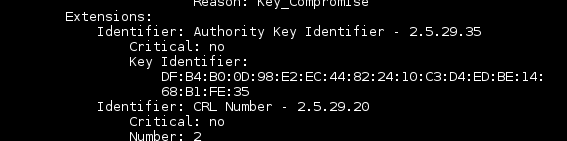
\includegraphics[width=65mm]{crl-aki.png}
                                    \caption{CRL Authority Key identifier}
                                \end{figure}
                        \end{itemize}
                \end{itemize}
            \item \textbf{Issuer Alternative Name}
                \begin{itemize}
                    \item This extension allows additional identities to be associated with the issuer or CRL.
                \end{itemize}
            \item \textbf{CRL Number}
                \begin{itemize}
                    \item This is a non critical extension that specifies sequence number for a given CRL scope and issuer. 
                    \item This extension allows users to determine if a particular CRL supersedes another CRL. 
                    \item if a CRL issuer generates delta CRLs in addition to complete CRLs for a given scope, the complete CRLs and delta CRLs must share one numbering sequence. 
                \end{itemize}
            \item \textbf{Delta CRL Indicator}
                \begin{itemize}
                    \item Delta CRL indicator is a critical CRL extension that identifies a CRL beging a delta CRL. 
                    \item Delta CRLs contain updates to the revocation information previously 
                        distributed, rather than all the information that would appear in 
                        complete CRL.
                    \item This helps in reducing network load and processing time in certain
                        environments
                    \item Example:
                        \begin{itemize}
                            \item \begin{figure}[ht!]
                                    \centering
                                    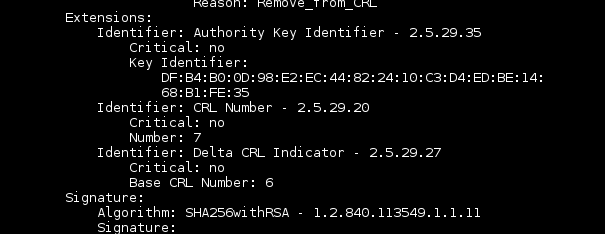
\includegraphics[width=80mm]{delta-crl-extension.png}
                                    \caption{Delta CRL Indicator Extension}
                                \end{figure}
                        \end{itemize}
                \end{itemize}
            \item \textbf{Issuing Distribution Point}
                \begin{itemize}
                    \item This is a critical CRL extension that identifies the CRL distribution point and scope for a particular CRL. 
                    \item It indicates whether CRL covers revocation of EE Certificates only, CA certificates etc. 
                    \item Example:
                        \begin{itemize}
                            \item \begin{figure}[ht!]
                                    \centering
                                    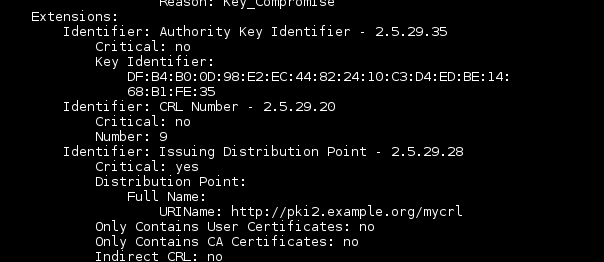
\includegraphics[width=80mm]{issuing-distribution-point.png}
                                    \caption{Issuing Distribution Point extension}
                                  \end{figure}
                        \end{itemize}
                \end{itemize}
    \end{itemize}
    \subsection{Mozilla NSS}
        \subsubsection{Introduction}
            \begin{itemize}
                \item RHEL has 3 sets of security libraries:
                        \begin{itemize}
                            \item OpenSSL
                            \item NSS
                            \item GnuTLS
                        \end{itemize}
                \item Network Security Services(NSS) is a project by Mozilla which provides crypto API majorly for Mozilla's products like 
                    \textit{Firefox}, \textit{Thunderbird}. 
                \item Mozilla NSS provides all the Public Key cryptography stands which other implementations provide. 
            \end{itemize}
        \subsubsection{Architecture}
            \begin{itemize}
                \item With default installation of RHEL, a NSS directory \textbf{/etc/pki/nssdb} is created for system wide usage. 
                \item Unlike openssl where certificates are created and stored in text files, certificates created by nss-tools are stored in nss database
                \item All certificates and keys  are stored in berkelely database(or SQLite). There are 3 major files generally seen in a nss directory are:
                    \begin{itemize}
                        \item \textbf{key3.db} file contains a key used to encrypt and decrypt saved passwords
                        \item \textbf{cert8.db} contains certificates
                        \item \textbf{secmod.db} contains pathnames of pkcs\#11 modules
                    \end{itemize}
             \end{itemize}
    \subsection{Exercises}
\begin{enumerate}[label*=\arabic*.]
    \item Setup: Create PKI Infrastructure using OpenSSL
        \begin{lstlisting}[style=BashInputStyle]
$ mkdir -p ~/pki/ca/{certs,crl,newcerts,private}
cd ~/pki/ca
chmod 700 private
touch index.txt
touch index.txt.attr
echo 01 > serial
wget https://raw.githubusercontent.com/mrniranjan/pkiworkshop/master/openssl.cnf
        \end{lstlisting}
    \item Create a CA cert using Openssl
        \begin{lstlisting}[style=BashInputStyle]
$ cd ~/pki/ca
$ openssl genrsa -out private/ca.key.pem 2048 -config openssl.cnf
$ chmod 400 private/ca.key.pem
$ openssl req -config openssl.cnf -key private/ca.key.pem -new -x509 \
    -days 365 -extensions v3_ca -out certs/ca.cert.pem
        \end{lstlisting}
    \item Create a End User cert with CN=Pki User1
        \begin{lstlisting}[style=BashInputStyle]
# Create a private key
        
$ cd ~/pki/ca
        
$ openssl genrsa -out private/pkiuser1.key 2048
        
# Create Certificate Request

$ openssl req -new -key private/pkiuser1.key \
    -out pkiuser1.csr -config openssl.cnf
        
$ openssl ca -config openssl.cnf -extensions usr_cert \
     -days 375 -in pkiuser1.csr -out certs/pkiuser1.cert.pem
        \end{lstlisting}
    \item Create a User cert \textit{cn=Pki User1} with adding extension "Authority Key Identifier" where 
        extension adds the hash of CA public key

        Add the below lines to \textbf{usr\_cert} section of openssl.cnf
        \begin{lstlisting}
basicConstraints=CA:FALSE
subjectKeyIdentifier=hash
authorityKeyIdentifier=keyid
        \end{lstlisting}
    \item Create a user cert by adding followin extensions digitalSignature, nonRepudiation

        Add the below lines to \textbf{user\_cert} section of openssl.cnf
        \begin{lstlisting}
keyUsage = nonRepudiation, digitalSignature
        \end{lstlisting}

    \item create a server cert by adding following extensions:

        Add the below  lines to \textbf{server\_cert} section of openssl.cnf
        \begin{lstlisting}
keyUsage = keyAgreement, digitalSignature
        \end{lstlisting}
    
    \item Create a user cert with subjectAltname having an email address

        Add the below lines to \textbf{user\_cert} section of openssl.cnf
        \begin{lstlisting}
subjectAltName = email:copy
        \end{lstlisting}

    \item create a CA cert with pathlength of 2 . Verify path validation by creating multiple CAs

        Create a new section \textbf{v3\_usr\_ca} in openssl.cnf and create certs
        \begin{lstlisting}
subjectKeyIdentifier=hash
authorityKeyIdentifier=keyid
basicConstraints = critical,CA:true,pathlen:2
keyUsage = cRLSign, keyCertSign
        \end{lstlisting}
    
    \item Create a server cert with TLS server and client authentication

        Create a new section \textbf{server\_cert} in openssl.cnf with below contents
        \begin{lstlisting}
[ server_cert ]
basicConstraints=CA:FALSE
subjectKeyIdentifier=hash
authorityKeyIdentifier=keyid
keyUsage = digitalSignature, keyAgreement
extendedKeyUsage = serverAuth,clientAuth
        \end{lstlisting}

    \item create a server cert with subject CN=server2.example.org having subjectAltName *.example.org
        
        Add below line to \textbf{server\_cert} section and create a new section \textbf{alt\_names}
        \begin{lstlisting}
[ server_cert ]
subjectAltName = @alt_names

[alt_names]
DNS.1 = *.example.org
       \end{lstlisting}

    \item Create a Name constraint where permitted DN attribute is "CN=pki*,OU=PKI,O=Example Org,C=US"

            Add below lines to \textbf{v3\_usr\_ca} 
            \begin{lstlisting}
[ v3_usr_ca ]
subjectKeyIdentifier=hash
authorityKeyIdentifier=keyid
basicConstraints = critical,CA:true,pathlen:0
keyUsage = cRLSign, keyCertSign
nameConstraints = permitted;dirName:dir_sect

[dir_sect]
C=IN
O=Example Org
OU=PKI
CN=*
            \end{lstlisting}
    \item Creating Certificate and key databases using NSS 
        \begin{itemize}
            \item Create the below structure of directories to store CA, Server and user certificates
                \begin{itemize}
                    \item \textbf{/etc/pki/nssdb/CA\_db} (for storing root CA certificates)
                    \item \textbf{/etc/pki/nssdb/server\_db} (for storing certificates of servers)
                    \item \textbf{/etc/pki/nssdb/client\_db} (for storing certificates of users)
                \end{itemize}
            
            \item create a new certificate database CA\_db
                \begin{lstlisting}[style=BashInputStyle]
$ cd /etc/pki/nssdb
$ mkdir CA_db
$ certutil -N -d CA_db
                \end{lstlisting}
            \item Create a Self signed Root CA certificate, specify the subject name
                \begin{lstlisting}[style=BashInputStyle]
$ certutil -s -d CA_db -n "Example RootCA" -s "CN=Example RootCA,OU=IDMQE,O=Example Org,L=Pune,ST=Maharashtra,C=IN" -t "CT,," -x -2
                \end{lstlisting}
                Explanation of the flags:
                \begin{lstlisting}
-S specifies create a individual certificate and add it to the database
-d specifies the directory of the nss database ( -d .  specifies current directory)
-n "Name of the certificate"
-t "CT,,"  specifies that this certificate is a Trusted CA which can issue server certficates
-x use the certutil tool to generate the signature for certificate being created or added to the database rather than obtaining from separate CA
-2 specifies that add basic constraint extensions,  like the certificate can be used to sign specific operations like SSL, opbject signing, SMIME
                \end{lstlisting}
            \item Extract the CA certificate from CA's cert database to a file
                \begin{lstlisting}[style=BashInputStyle]
$ certutil -L -d CA_db -n "Example RootCA" -a -o rootca.crt
                \end{lstlisting}
            \item Display the contents fot the CA's Certificate database
                \begin{lstlisting}[style=BashInputStyle] 
$ certutil -L -d .
                \end{lstlisting}
            \item Creating Certificates for Servers, For servers SSL servers or clients
                \begin{lstlisting}[style=BashInputStyle]
$ mkdir /etc/pki/nssdb/server_db
$ certutil -N -d server_db
                \end{lstlisting}
            \item Import the new CA certificate in the Server certificate's database and we mark it as trusted CA
                \begin{lstlisting}[style=BashInputStyle]
$ certutil  -A -d server_db -n "Example CA" -t "TC,," -a -i CA_db/rootca.crt
                \end{lstlisting}
            Explanation of the flags:
                \begin{lstlisting}
-A Add an existing certificate to a certificate database
-d server_db  (directory of certificate database)
-t "TC", specifies that this certificate is a Trusted CA which can issue server certficates, client certificates. ",," specifies  uu i.e "CT,u,u" , where u specifies certificate can be used
-a is ascii format
-i input file
                \end{lstlisting}
            \item Create the server certificate request, specifying the subject name for the server certificate. Generally CN should be identical to the hostname of the server
                \begin{lstlisting}[style=BashInputStyle]
$ certutil -R -d server_db  -s "CN=pki1.example.org,OU=IDMQE,O=Example Org,L=Pune,ST=Maharashtra,C=IN" -a -o server_db/pki1.req -v 12
                \end{lstlisting}
            \item Sign the Certificate from CA , and  issues a  new certificate in ascii format

                \begin{lstlisting}[style=BashInputStyle]
$ certutil -C -d CA\_db -c "Example RootCA" -a -i server_db/pki1.req -o server_db/pki1.pem -2 -6
                \end{lstlisting}

            \item Import (Add) the new server certificate to the server's certificate database in the server\_db directory with appropriate nickname
                 \begin{lstlisting}[style=BashInputStyle]
$ certutil -A -d server_db -n pki1 -a -i server_db\pki1.pem -t ",,"
                 \end{lstlisting}

            \item View the certificate
                \begin{lstlisting}[style=BashInputStyle]
$ certutil -V -d server_db -u V -n pki1
                \end{lstlisting}

            \item By default the certificates that have been created using the above procedure are in pkcs12 standard to use the certificates on Applications,  You would require the following
                \begin{itemize}
                    \item RootCA's Certificate (public key)
                    \item Server Certificate (Certificate and key). The Server's participating in SSL communication should have the certificates and key file
                \end{itemize}

            \item nss-tools comes with pk12util command , pk12util is a pkcs\#12 Tool allowing to share certificates. The tool supports importing certificates and keys from pkcs\#12 files in to NSS or export them and also list certificates and keys in such files

            \item Exporting the Server certifcate pki1.example.org in to file pki1.p12 
                \begin{lstlisting}[style=BashInputStyle]
$ pk12util -d server_db -o pki1.pk12 -n pki1
                \end{lstlisting}

            \item The Above pki1.pk12 file has both the certificate and the key file encrypted

            \item For Applications which require certificate and key file to be in pem format we can use Openssl command to convert the file from \.p12 to pem format.
                \begin{lstlisting}[style=BashInputStyle]
$ openssl pkcs12 -clcerts -nokeys -in pki1.pk12 -out pki1.pem
$ openssl pkcs12 -nocerts -in pki1.pk12 -out pki1.key.pem -nodes
                \end{lstlisting}
        \end{itemize}
\end{enumerate}
\section{Common Terms Used in RHCS}
\begin{itemize}
    \item Enrollment
        The point when the certificate is issued to the User/client is called enrollment
    \item Renewal
        When certificate is about to be expired or already expired and has CA requires to 
        renew the certificate
    \item Dual Keys
        Conventional hierarchical PKI uses a single key pair – one public key and one
        private key. According to VeriSign, “Key Pairs are used for one or more of three basic purposes:
        \begin{itemize}
            \item Encryption
            \item Authentication
            \item non-repudiation
        \end{itemize}
         A single key used for multiple purposes violates non-repudiation.
         It is recommended that you assign two key pairs per person -- one key pair for signing messages 
         providing authentication and non-repudiation, and a second key pair for encryption. 
         This allows someone to recover the encryption key and decrypt documents that were encrypted using it,
         without their gaining the ability to sign documents with that user’s private key as well (which
         could lead to forgery and violation of non-repudiation)
    \item ECC
        is a cryptographic system that uses elliptic curves to create keys for encrypting data. 
        ECC creates cryptographically-stronger keys with shorter key lengths  than RSA, which makes it faster 
        and more efficient to implement. But it is not widely supported as RSA
    \item CRMF
        Certificate Request Message Format is a syntax use to convey a request for a certificate to Certificate
        Authority (CA). This request contains a public key, Proof of Possession(POP), Additional registration informtion
        combined with pop and public key.\cite{4211}
    \item PKCS10 
        is a standard which specifies syntax for Certificate Request. A certificate request consists of: ~\cite{2986}
        \begin{itemize}
            \item Dishtinguished Name
            \item Public Key
            \item Optional Set of attributes
        \end{itemize}
    \item FIPS
        Federal Information Processing Standards (FIPS) are standards to be followed by US Federal Govt for use in system by non-military govt. agencies and contractors.  
    \item FIPS-140
        standard specifies the security requirements for a cryptographic module utilized within a security system protecting sensitive information in computer and telecommunication systems. US national Institute of Standards and Technology(NIST) publishes FIPS series of standards for the implementation of Cryptographic modules. Cryptographic Module Validation Program (CMVP) validates cryptographic modules to Federal Information Processing Standard (FIPS) 140-2 and other cryptography based standards. 

        FIPS 140-2 is primarily of interest to U.S., Canadian, and UK government agencies which have formal policies requiring use of FIPS 140 validated cryptographic software. ~\cite{nist:fips}

        Products that have received a NIST/CSE validation are listed on the Cryptographic Module Validation List : http://csrc.nist.gov/groups/STM/cmvp/documents/140-1/140val-all.htm
    \item HSM
        is a physical computing device that safeguards and manages digital keys for strong authentication and provides cryptoprocessing. HSM's are used in PKI environment. HSM's are designed to protect keys(private). A private key in HSM cannot be extracted.     
\end{itemize}
\section{Red Hat Certificate System}
    \begin{itemize}
        \item RHCS is an Enterprise PKI implementation providing various PKI operations like Enrollment, renewal, revocation
        \item Provides Certificate Lifecycle Management  like CA, Key archival, smartcard management. 
        \item Key Features:
            \begin{itemize}
                \item Certificate issuance, revocation, and retrieval 
                \item Certificate Revocation List (CRL) generation and publishing
                \item Certificate profiles
                \item Encryption key archival and recovery 
                \item Smartcard lifecycle management 
            \end{itemize}
    \end{itemize}
\subsection{Overview}
    RHCS Comprises of 5 subsystems each providing a set of PKI operations:
    \begin{itemize}
        \item Certificate Manager:Also called Certificate Authority is the core of PKI.
            \begin{itemize}
                \item Issues certs
                \item Revokes Certs
                \item Publishes CRL
                \item Establishes Security Domain of trusted subsystems
            \end{itemize}
        \item Key Recovery Authority(KRA):It's also called Data Recovery Manager(DRM) 
            \begin{itemize}
                \item where private key is archived for certificates which have been created based on unique pair. 
                \item KRA archives the key pair and can later be retrieved if the private key of the certificate is lost
            \end{itemize}
        \item Online Certificate Status Protcol(OCSP): 
            \begin{itemize}
                \item OCSP Verifies certificate is valid or not expired
            \end{itemize}
        \item Token Processing System(TPS)
            \begin{itemize}
                \item TPS interacts with smartcard and manages keys and certificates on those tokens. TPS to interact
                    with Smartcard it takes help of Token Key service which creates keys to interact with smartcard securely
            \end{itemize}
        \item Token key System(TKS)
            \begin{itemize}
                \item TKS derives keys based on the token CCID, private information,and a defined algorithm. 
                    These derived keys are used by the TPS to format tokens and enroll, or process, certificates on the token.
            \end{itemize}
        \item Enterprise Security Client(ESC)
            \begin{itemize}
                \item ESC is software installed on client systems which have tokens connected to it.
                \item ESC is used to enroll, format smartcard 
                \item TPS talks to ESC to insert certificates in to smartcards.
            \end{itemize}
    \end{itemize}
    \begin{figure}[H]
        \centering
        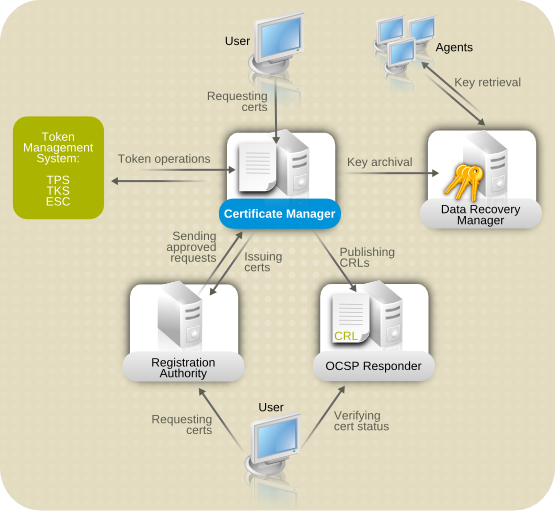
\includegraphics[width=80mm]{rhcs-subsystem-overview.png}
        \caption{RHCS Subsystems ~\cite{RedHat:CSoverview}}
    \end{figure}
\subsection{Version}
    \subsubsection{Older Versions}
        \begin{itemize}
            \item Red Hat Certificate System 7.2 (2006) 
            \item Red Hat Certificate System 7.3 (2007)
        \end{itemize}
    \subsubsection{Current Version}
        \begin{itemize}
            \item Red Hat Certificate System 8 (2009) 
                \begin{itemize}
                    \item Support Status: Maitainance Support July 22, 2014 – July 03, 2017 
                \end{itemize}
            \item Red Hat Certificate System 9 (2015)
                \begin{itemize}
                    \item Full support (including hardware updates): September 02, 2015 – September 02, 2018
                \end{itemize}
        \end{itemize}
\subsection{Builds}
    \subsubsection{Architecture}
        \begin{itemize}
            \item RHCS8 is supported in below architectures:
                \begin{itemize}
                    \item x86\_64
                    \item i686
                \end{itemize}
            \item RHCS9 is supported in x86\_64 only
        \end{itemize}
    \subsubsection{Builds}
        \begin{itemize}
            \item RHCS8 Brew Tags:
                \begin{itemize}
                    \item certsys-8-advanced-rhel-5-candidate
                \end{itemize}
            \item RHCS9 Brew Tags:
                \begin{itemize}
                    \item pki-9-rhel-7-candidate [QE Build]
                \end{itemize}
            \item RHCS9 Builds
                \begin{itemize}
                    \item pki-core-10.2.6.9.el7pki , which provides:
                        \begin{itemize}
                            \item pki-ca
                            \item pki-kra
                            \item pki-ocsp
                            \item pki-tks
                            \item pki-tps
                            \item pki-symkey
                            \item pki-base
                            \item pki-javadoc
                            \item pki-tools
                            \item pki-server
                        \end{itemize}
                    \item pki-console-10.2.6-1.el7pki
                    \item redhat-pki-10.2.6-1.el7pki
                    \item redhat-pki-theme-10.2.6-1.el7pki
                \end{itemize}
        \end{itemize}
\subsection{Features}
    Some of Key Features of RHCS9 are: 
    \begin{itemize}
        \item RHCS 9 continues to support separate PKI instances for all subsystems
        \item RHCS 9 introduces the notion of a shared PKI instance:
        \item \textit{pkispawn} CLI to install and configure new PKI subsystems, support both 
            interactive and batch mode or combination of both.
        \item \textit{pkidestroy} CLI to remove PKI instance
        \item RHCS9 services are managed using systemd 
            \begin{itemize}
                \item systemctl [start|status|stop|restart] pki-tomcatd@$<$instance$>$.service
            \end{itemize}
        \item RHCS9 Process management can be done using cli \textit{pki-server} and \textit{pkidaemon}
        \item Support for REST Web Services APIs
        \item Web User Interface (UI) Customization
        \item New Command-Line Interface (CLI) Utilities
    \end{itemize}
\subsection{Certificate Manager}
\subsubsection{Introduction}
Certificate Manager is the first subsystem that needs to be configured in PKI Environment, Certificate Manager can be configured as RootCA, Subordinate CA
\subsubsection{Installation}
    \begin{itemize}
        \item RPM: \textrm{\textbf{pki-ca}}
        \item configuration:  CA subsystem is configured using utility \textbf{pkispawn}. 
            
            pkispawn provides both interactive configuration  or silent configuration by reading a configuration file. 
            
            pkispawn first reads \textbf{default.cfg} first and gets other deployment specific information through interactive method
            or through batch mode by reading a file. 

            pkispawn then passes this information to a java servlet which performs the configuration. 
        \begin{figure}[ht!]
            \centering
            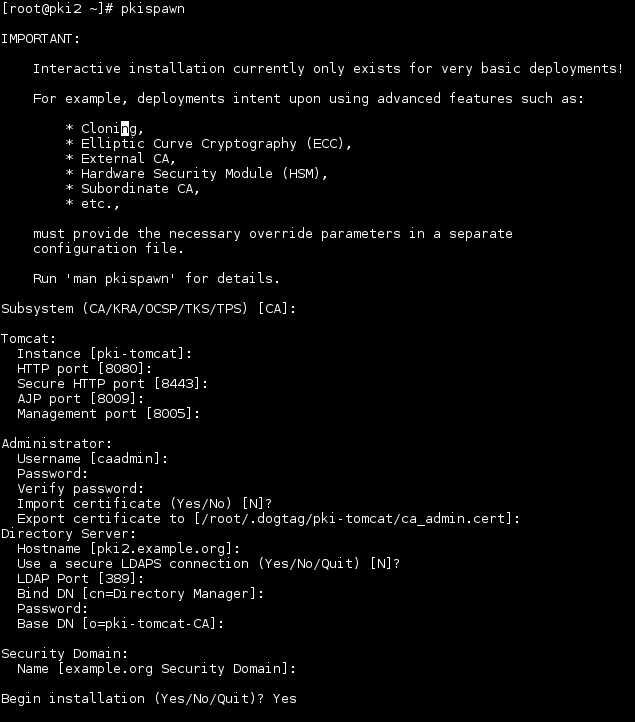
\includegraphics[width=65mm]{pkispawn-ca.png}
            \caption{Configuring CA subsystem using pkispawn}
        \end{figure}
    \end{itemize}
\subsubsection{Installation Layout}
    \begin{itemize}
        \item \textbf{/var/lib/pki/$<$instanceName$>$}: <Instance> here is the tomcat Instance name given during configuring subsystem
        \item \textbf{/var/lib/pki/$<$instance$>$/alias}: Is the NSS Database of the system where the subsystem system certs are stored.
            When a subsystem is configured, Certain certificates are created for certain tasks like audit signing, OCSP Signing, CA Signing cert.
            These system certificates reside in alias directory. List of system certs are mentioned below, All the below system certs are issued by
            CA during configuration of CA.
            \begin{itemize}
                \item caSigningCert (\textit{Used to sign Certs})
                \item Server-Cert (\textit{Certificate of the server having CA})
                \item auditSigningCert (\textit{Certificate used to sign Audit messages})
                \item subsystemCert (\textit{Subsystem Certificate})
            \end{itemize}
        \item \textbf{/var/lib/pki/$<$instance$>$/conf:} Configuration directory containing
            tomcat configuration, password file containing internal database(ldap) password, 
            and NSS Database password
        \item \textbf{/var/lib/pki/$<$instance$>$/ca/:} Contains CA Subsystem configuration 
                file CS.cfg. This file is the main configuration file for CA subsystem
    \end{itemize}
\subsubsection{Key Features}
    \begin{itemize}
        \item CA subsystem issues, renews, revokes Certificates, generates Certificat Revocation lists
        \item Publishes Certificates/CRL in form of files or can publish to LDAP or OCSP responder
        \item CA also has an inbuilt OCSP responder enabling OCSP-Compliant clients to query CA about revocation status of Certificate
        \item Some CA's can delegate some of it's responsibility to another Subordinate CA
    \end{itemize}
\subsubsection{Architecture}
     \begin{figure}[H]
          \centering
          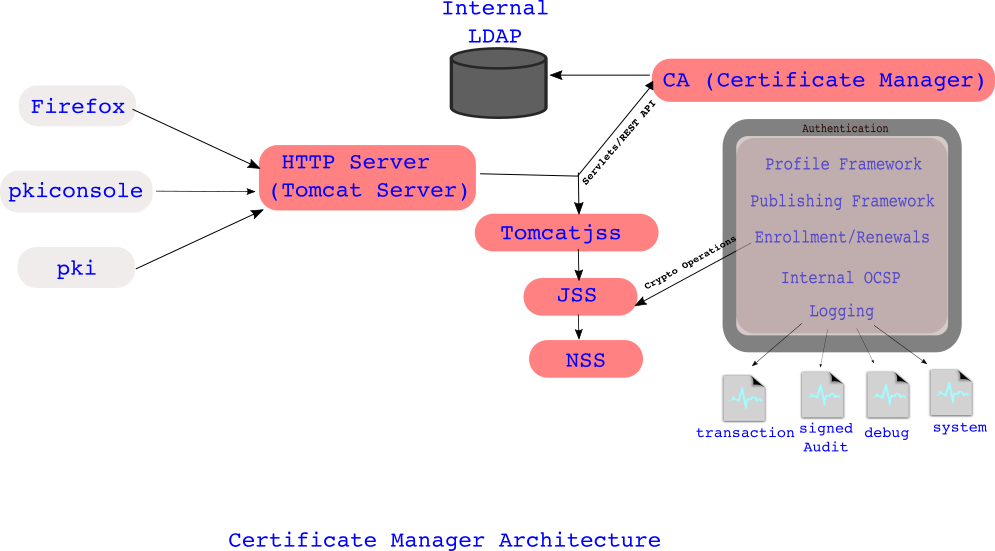
\includegraphics[width=80mm]{CA-subsystem-Arch3.png}
          \caption{CA Subsystem Architecture}
    \end{figure}
\subsubsection{Interfaces}
    \begin{itemize}
        \item End User Interface(Browser/CLI)
        \item Agent Interface(Browser/CLI)
        \item Admin interface(java console)
    \end{itemize}
\subsubsection{Features}
    \begin{itemize}
        \item Enrollment:

            End user Enrolls in the PKI infrastructure by submitting a Enrollment(certificate) request through End Entity Interface.
            This request can be submitted through 2 Methods:
            \begin{itemize}
                \item Browser
                \item CLI
            \end{itemize}
            There can be different kinds of Enrollment(Certificate) Request:
            \begin{itemize}
                \item Request for User, Server, SMIME, Dual Cert,.. certificate
                \item Request certificate if authentication through ldap, pin, cert etc. 
            \end{itemize}
            Based on the above types, there are different certificate profiles associated with it. 
            When end-entity(user) enrolls a certificate following events occur:
            \begin{itemize}
                \item The End-entity provides the information in one of the enrollment forms and submits a request
                \item The enrollment forms triggers the creation of public-key and private-key or dual-key pairs
                \item The End-entity provides authentication credentials before submitting the request,
                     depending on the authentication type. This can be LDAP authentication, PIN-based authentication or certificate-based authentication.
                \item The request is submitted either to an agent-approved enrollment process or an automated process.
                    \begin{itemize}
                        \item Agent-approved process requires no end-entity authentication, sends the request to the request queue in the agent-services interface.
                        \item Automatic notification can be setup so an email can be sent to an agent any time a request appears in the queue
                        \item The automated process, which involves end-entity authentication,process the certificate as soon as the end-entity successfully authenticates
                    \end{itemize}
                \item This form collects information about the end entity from the LDAP directory when the form is submitted
                \item The profile associated with form determine the aspects of certificate that is issued. Depending upon the certificate profile the request is evaluated to determine if the request meets the constraints set.
                \item The Certificate request is either rejected because it did not meet the certificate profile or authentication requirement, or a certificate is issued
                \item The certificate is delivered to end-entity  through HTML interface or email or certificate can be retrieved through Agents interface by serial number or request-ID.
                \item The new certificate is stored in Certificate Managers internal database.
                    \begin{figure}[ht!]
                    \centering
                    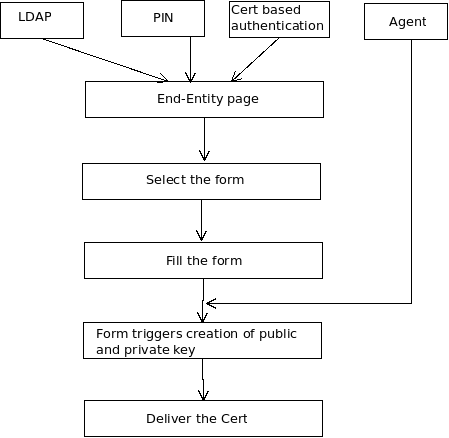
\includegraphics[width=35mm]{enrollment.png}
                    \caption{Certificate Enrollment}
                    \end{figure}
                \end{itemize}
        \item Profiles:

            Profile determine the content of a certificate. Certificate manager provides customizable framework to apply 
            policies for incoming certificate requests and to control the input requests types and output certificate types

            Certificate Profile define the following:
            \begin{itemize}
                \item  Authentication Method
                \item  Authorization Method
                \item  Certificate content
                \item  Constraints for the values of content
                \item  Contents of input
                \item  Output
            \end{itemize}
            \begin{figure}[ht!]
                \centering
                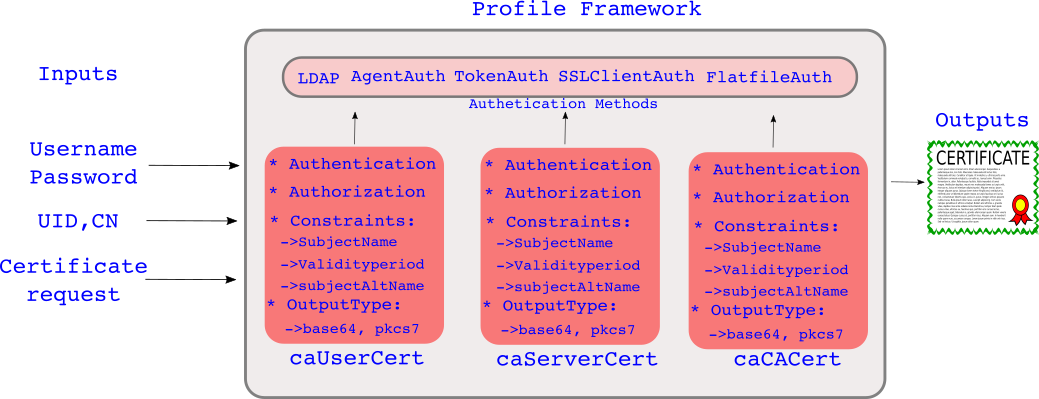
\includegraphics[width=90mm]{CA-profiles-arch.png}
                \caption{Certificate Profile Architecture}
            \end{figure}
            Profile Workflow:
            \begin{figure}[ht!]
                \centering
                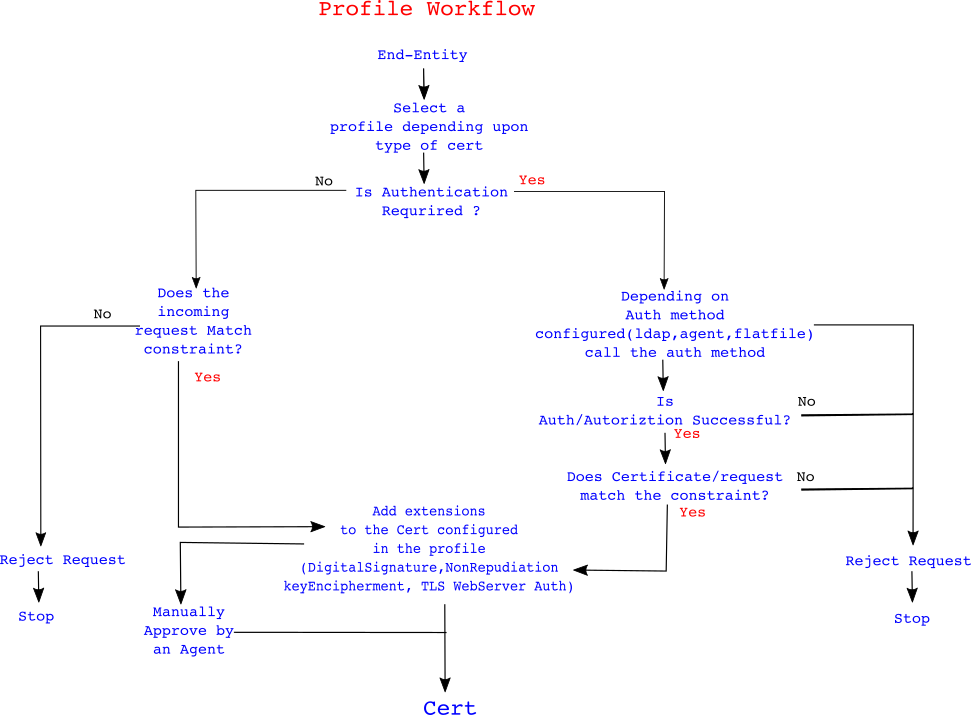
\includegraphics[width=80mm]{CA-Profiles-workflow.png}
                \caption{Certificate Profiles Workflow}
            \end{figure}
            
            Each profile are defined in \textbf{.cfg} file located at \textbf{/var/lib/instance\_name/profiles/ca} directory

            Example \textbf{caUserCert} Profile:

            The first part of the profile is the description and specifies whether profile is enabled or disabled, if enabled who
            enabled it. 
            \begin{figure}[ht!]
                \centering
                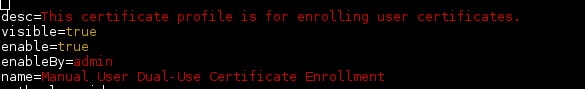
\includegraphics[width=80mm]{profile-1.png}
                \caption{Profile Description}
            \end{figure}
            
            The second part of the profile describes the inputs:
            \begin{figure}[ht!]
                \centering
                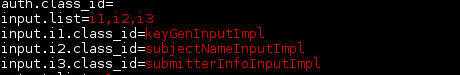
\includegraphics[width=80mm]{profile-2.png}
                \caption{Profile inputs}
            \end{figure}
            \begin{itemize}
                \item \underline{KeyGenInputImpl}: specifies the key pair generation during the request submission, This provides if the request
                    should be of type CRMF/PKCS10, also provides dropdown specifying the key size.
                \item \underline{subjectNameInputImpl}: specifies the subject Distinguished Name(DN) to be used in the cert. The subject DN 
                    can be constructed from \textit{UID, Email, Common Name, Organizational Unit, Country}
                \item \underline{submitterInfoImpl}: This input specifies three fields: \textit{Requester Name, Requester email, Requester phone}
            \end{itemize}
            \begin{figure}[ht!]
                \centering
                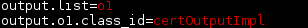
\includegraphics[width=80mm]{profile-3.png}
                \caption{Profile output}
            \end{figure}
            Third part of the profile is output, 
            \begin{itemize}
                \item \underline{certOutputImpl}: The certificate output format \textit{base64, pkcs7, prettyprint}
            \end{itemize}
            \begin{figure}[ht!]
                \centering
                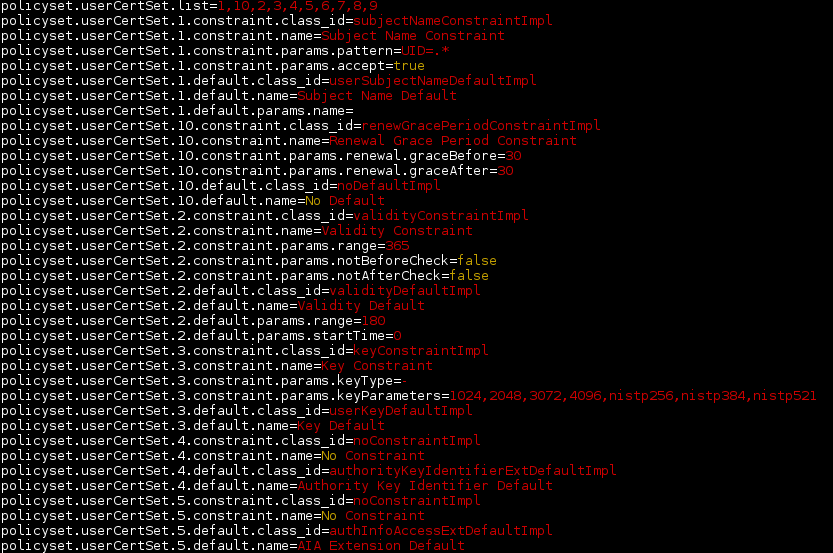
\includegraphics[width=80mm]{profile-4.png}
                \caption{Profile Policies}
            \end{figure}

            Last part of the profile is constraints, Policies like:
            \begin{itemize}
                \item validity of the cert
                \item renewal settings, 
                \item key Usage Extensions
                \item User supplied extensions
            \end{itemize}
        \item Publishing 
            Certificate System provides customizable framework from CA's to publish.
            \begin{figure}[h!]
                \centering
                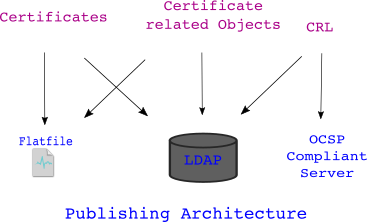
\includegraphics[width=40mm]{publishing3.png}
                \caption{Publishing Architecture}
            \end{figure}
            \begin{itemize}
                \item Key Features
                    \begin{itemize}
                        \item Publish to a single repositories or multiple repositories
                        \item Split locations by certificates/CRL
                        \item Set individual rules for each type of certs/crl
                    \end{itemize}
                \item Publishing framework consists
                    \begin{itemize}
                        \item Publishers
                        \item Mappers
                        \item Rules
                    \end{itemize}
                \item \underline{Publishers:}
                    Publishers specify location to which certificates/CRL's are to be published. 
                        Example: 
                        \begin{itemize}
                            \item To publish to a file, publishers specify the location of the publishing directory.
                            \item To publish to LDAP, publishers specify the attribute in the directory that srores the cert/CRL.
                            \item To publish to OCSP, we specify OCSP Server details. 
                        \end{itemize}
                    \item \underline{Rules}: Rules define 
                        \begin{itemize}
                            \item what is to be published and where ?
                            \item What type of certs can be published to what location
                            \item Set rules to publish certs to file and LDAP
                            \item Set individual rules for each type of cert/rule
                            \item There are rules for Files, LDAP and OCSP
                        \end{itemize}
                    \item \underline{Mappers}: Mappers are only used when publishing to LDAP
                        \begin{itemize}
                            \item Mappers construct the DN for an entry based on the information
                                from the certificate or certificate request. 
                            \item Mappers use certificate or certificate request's subject name to
                                construct the DN of the entry to which cert/certificate request/CRL has to be published
                        \end{itemize}
            \end{itemize}
    \end{itemize}
\subsubsection{Exercises}
    \begin{enumerate}[label*=\arabic*.]
        \item \label{setup1} Require 2 RHEL7/Fedora 23 systems , setup hostnames as specified below and make setup hostname
            resolutions through \textit{/etc/hosts}:
            \begin{lstlisting}
pki1.example.org
pki2.example.org
            \end{lstlisting}
        \item \label{setup2} Configure vncserver on both systems
        \item \label{setup3} Setup CS9 and RHEL7 Optional Repos
            \begin{lstlisting}[style=BashInputStyle]
$ cat /etc/yum.repos.d/rhcs9.repo

[rhcs9]
name=Red Hat Certificate Services 9
baseurl=http://download.eng.bos.redhat.com/rcm-guest/puddles/RHCS/9.0.1/latest/x86_64/os/
enabled=1   
gpgcheck=0

$ cat /etc/yum.repos.d/rhel7-optional.repo

[rhel7-optional]
name=Red Hat Enterprise Linux 7.2 Optional
baseurl=http://download.eng.pnq.redhat.com/released/RHEL-7/7.2/Server-optional/x86_64/os/
enabled=1
gpgcheck=0
            \end{lstlisting}

        \item \label{setup4} Setup Install \textbf{\textit{redhat-pki}} and \textbf{\textit{389-ds-base}} package 

            \begin{lstlisting}[style=BashInputStyle]
$ yum install redhat-pki
$ yum install 389-ds-base
            \end{lstlisting}
        
        \item \label{rootca} Setup CA Subsystem using pkispawn in interactive mode
            \begin{enumerate}[label*=\arabic*.]
                \item \label{ds1} Setup Directory Server in silent mode by specify config parameters in file 
                    \begin{lstlisting}[style=bashInputStyle]
$vim ca-ds.inf
[General]
FullMachineName=pki1.example.org 
SuiteSpotUserID=nobody
SuiteSpotGroup=nobody

[slapd]
ServerIdentifier=Example1-RootCA
ServerPort=389
Suffix=dc=example,dc=org
RootDN=cn=Directory Manager
RootDNPwd=Secret123

[admin]
ServerAdminID=admin
ServerAdminPwd=Secret123
SysUser=nobody
                    \end{lstlisting}
                    \begin{lstlisting}[style=bashInputStyle]
$ setup-ds.pl --silent --file=ca-ds.inf --debug
                    \end{lstlisting}
                \item \label{ca1}Run \textbf{\textit{pkispawn}} in interactive mode use default ports and specify Directory
                    server information configured above. Use Tomcat Instance name as 'pki-tomcat'
                    \begin{lstlisting}
Subsystem (CA/KRA/OCSP/TKS/TPS) [CA]:

Tomcat:
  Instance [pki-tomcat]:
  HTTP port [8080]:
  Secure HTTP port [8443]:
  AJP port [8009]:
  Management port [8005]:

Administrator:
  Username [caadmin]:
  Password:
  Verify password:
  Import certificate (Yes/No) [N]?
  Export certificate to [/root/.dogtag/pki-tomcat/ca_admin.cert]:
Directory Server:
  Hostname [pki1.example.org]:
  Use a secure LDAPS connection (Yes/No/Quit) [N]?
  LDAP Port [389]:
  Bind DN [cn=Directory Manager]:
  Password:
  Base DN [o=pki-tomcat-CA]:

Security Domain:
  Name [example.org Security Domain]:

Begin installation (Yes/No/Quit)? Yes
                    \end{lstlisting}
            \end{enumerate}
        \item \label{ca2} Setup Subordinate CA to the CA configured in \ref{ca1} within the same security domain as RootCA
            \begin{enumerate}[label*=\arabic*.]
                \item Configure Directory server instance similar to \ref{ds1} but with different port and use instance name as Example1-SubCA
                \item Create a config file with below information to setup Subordinate CA or RootCA in same security Domain
                    \begin{lstlisting}
$ cat subca1.inf 

[DEFAULT]
pki_instance_name=Example1-SubCA1
pki_https_port=18443
pki_http_port=18080
pki_admin_password=Secret123
pki_client_database_password=Secret123
pki_client_pkcs12_password=Secret123
pki_ds_password=Secret123
pki_security_domain_password=Secret123
pki_security_domain_hostname=pki1.example.org
pki_security_domain_https_port=8443
pki_security_domain_user=caadmin

[Tomcat]
pki_ajp_port=18009
pki_tomcat_server_port=18005

[CA]
pki_subordinate=True
pki_issuing_ca=https://pki1.example.org:8443
pki_ca_signing_subject_dn=cn=CA Subordinate Signing,o=example.org
pki_ds_hostname=pki1.example.org
pki_ds_ldap_port=1389
pki_ds_password=Secret123
pki_ds_secure_connection=False
                    \end{lstlisting}
                \item  Run pkispawn with above configuration to configure SubCA.
                    \begin{lstlisting}[style=bashInputStyle]
$ pkispawn -s CA -f subca1.inf -vv
                    \end{lstlisting}
                \item Verify Subsystem status using systemctl and pkidaemon commands
                    \begin{lstlisting}[style=bashInputStyle]
$ systemctl status pki-tomcatd@Example-SubCA1
$ pkidaemon status tomcat Example1-SubCA1
                    \end{lstlisting}
                \end{enumerate}
            \item \label{ca3} Configure External CA signed by RootCA configured in \ref{ca1}
                \begin{enumerate}[label*=\arabic*.]
                    \item Configure Directory server instance similar to \ref{ds1} but with different port and use instance name as Example1-SubCA2
                        \begin{lstlisting}
$vim ca-ds.inf

[General]
FullMachineName=pki1.example.org 
SuiteSpotUserID=nobody
SuiteSpotGroup=nobody

[slapd]
ServerIdentifier=Example1-ExtCA1
ServerPort=2389
Suffix=dc=example,dc=org
RootDN=cn=Directory Manager
RootDNPwd=Secret123

[admin]
ServerAdminID=admin
ServerAdminPwd=Secret123
SysUser=nobody
                        \end{lstlisting}            
                    \item \label{ca3.1} Setting up External CA is 2 step process.  In the first step, a certificate signing request (CSR) 
                    is generated for the signing certificate and ca-ext.inf contains the following text:
                        \begin{lstlisting}
$ vim ca-ext.inf 

[DEFAULT]
pki_instance_name=Example1-ExtCA1
pki_https_port=30042
pki_http_port=30044
pki_admin_password=Secret123
pki_client_database_password=Secret123
pki_client_pkcs12_password=Secret123
pki_ds_password=Secret123
pki_security_domain_password=Secret123

[Tomcat]
pki_ajp_port=30009
pki_tomcat_server_port=30005

[CA]
pki_external=True
pki_external_csr_path=/tmp/ca_signing.csr
pki_ca_signing_subject_dn=cn=CA Signing,ou=External,o=example.org
pki_ds_hostname=pki1.example.org
pki_ds_ldap_port=2389
pki_ds_password=Secret123
pki_ds_secure_connection=False
                        \end{lstlisting}
                    \item \label{ca3.2} issue pkispawn command with the above file and this creates a certificate request at location \textit{/tmp/ca\_signing.csr}
                        \begin{lstlisting}[style=bashInputStyle]
$ pkispawn -s CA -f ca-ext.inf -vv
                        \end{lstlisting}
                    \item Verify subsystem status using systemctl and pkidaemon commands
                    \begin{lstlisting}[style=bashInputStyle]
$ systemctl status pki-tomcatd@Example-SubCA1
$ pkidaemon status tomcat Example1-SubCA1
                    \end{lstlisting}
                    \item Get the certificate request signed by RootCA configured in \ref{ca1}
                    \item Import CA Admin cert to firefox and Approve the request using belwo procedure:
                        \begin{itemize}
                            \item Access CA EE interface
                            \item Copy the certificate request and submit using the profile:
                                    "Manual Certificate Manager Signing Certificate Enrollment"
                            \item From Agent interface approve the request
                            \item Copy the Approved cert and save it to a file /tmp/ca\_signing.cert
                            \item Also copy the CA cert chain and save it to file /tmp/ca\_cert\_chain.cert
                        \end{itemize}
                    \item Edit ca-ext.inf as show below
                        \begin{lstlisting}
[DEFAULT]
pki_instance_name=Example1-ExtCA1
pki_https_port=30042
pki_http_port=30044
pki_admin_password=Secret123
pki_client_database_password=Secret123
pki_client_pkcs12_password=Secret123
pki_ds_password=Secret123
pki_security_domain_password=Secret123

[Tomcat]
pki_ajp_port=30009
pki_tomcat_server_port=30005


[CA]
pki_external=True
pki_external_ca_cert_chain_path=/tmp/ca_cert_chain.cert
pki_external_ca_cert_path=/tmp/ca_signing.cert
pki_external_step_two=True
pki_ca_signing_subject_dn=cn=CA Signing Certificate,ou=External,o=example.org
pki_ds_hostname=pki1.example.org
pki_ds_ldap_port=2389
pki_ds_password=Secret123
pki_ds_secure_connection=False
                        \end{lstlisting}
                    \item Run pkispawn with above modified configuration file
                        \begin{lstlisting}[style=bashInputStyle]
$ pkispawn -s CA -f ca-ext.inf -vv 
                        \end{lstlisting}
                    \item Verify subsystem status using systemctl and pkidaemon commands
                    \begin{lstlisting}[style=bashInputStyle]
$ systemctl status pki-tomcatd@Example-ExtCA1
$ pkidaemon status tomcat Example1-ExtCA1
                    \end{lstlisting}
                \end{enumerate}
            \item \label{clone_rootca} Configure Clone of RootCA configured in \ref{ca1}
                \begin{enumerate}[label*=\arabic*.]
                    \item Features of clone
                        \begin{itemize}
                            \item A clone of subsystem is a replica of Master subsystem 
                            \item A cloned subsystem has same set of system certs including signing cert 
                            \item Clone acts as a load balancer
                        \end{itemize}
                    \item \label{pkcs12export} Create a Backup of RootCA's System Certs in pkcs12 format using PKCS12Export
                        \begin{lstlisting}[style=bashInputStyle]
$ PKCS12Export -d /var/lib/pki/pki-tomcat/alias -p /tmp/nssdb-pass  -w /tmp/pkcs12-pass -o ca_backup_keys.p12
                        \end{lstlisting}
                    \item Copy \textit{ca-backup.p12} to the Clone system
                    \item On clone system setup Directory Server using silent mode

ca-clone-ds.inf:                         
                        \begin{lstlisting}
[General]
FullMachineName=pki2.example.org
SuiteSpotUserID=nobody
SuiteSpotGroup=nobody

[slapd]
ServerIdentifier=Example1-Clone-CA1
ServerPort=389
Suffix=dc=example,dc=org
RootDN=cn=Directory Manager
RootDNPwd=Secret123

[admin]
ServerAdminID=admin
ServerAdminPwd=Secret123
SysUser=nobody                       
                        \end{lstlisting}
                    \item Setup Directory Server using \textit{setup-ds.pl} command
                        \begin{lstlisting}[style=bashInputStyle]
$ setup-ds.pl --silent --file=ca-clone-ds.inf --debug                    
                        \end{lstlisting}

                    \item Setup Clone using pkispawn
                    
                    \textbf{Note:} Clone configuration of RHCS subsystems cannot be done in interactive mode, hence requires
                    an input file containing all configuration parameters to be passed to pkispawn.

ca-clone-inst.inf:                    
                    \begin{lstlisting}
[DEFAULT]
pki_instance_name=Example1-CloneCA
pki_https_port=8443
pki_http_port=8080

#Admin
pki_admin_password=Secret123

#client Dir
pki_client_database_password=Secret123
pki_client_pkcs12_password=Secret123
pki_client_dir=/opt/Foobar1-CloneCA

#Security Domain
pki_security_domain_password=Secret123
pki_security_domain_hostname=pki1.example.org
pki_security_domain_https_port=8443
pki_security_domain_user=caadmin

[Tomcat]
pki_ajp_port=8009
pki_tomcat_server_port=8005

[CA]
pki_clone=True
pki_clone_pkcs12_password=Secret123
pki_clone_pkcs12_path=/tmp/ca_backup_keys.p12
pki_clone_replicate_schema=True
pki_clone_uri=https://pki1.example.org:8443
#Directory Server
pki_ds_password=Secret123
pki_ds_hostname=pki2.example.org
pki_ds_ldap_port=389
pki_ds_base_dn=o=Example1-RootCA-CA
pki_clone_replication_master_port=389
pki_clone_replication_clone_port=389
pki_ds_secure_connection=False
pki_ds_remove_data=True
                    \end{lstlisting}
                    \begin{lstlisting}[style=bashInputStyle]
$ pkispawn -s CA -f ca-clone-inst.inf -vv 
                    \end{lstlisting}
            \end{enumerate}
        \item Configure a Custom profile \textbf{\underline{caFoobarSanCert}} which generates cert with user provided SAN from CSR
                        along with CN from Subject DN
            \begin{enumerate}[label*=\arabic*.]
                \item Access pkiconsole of RootCA configured in \ref{ca1} using caadmin user
                    \begin{lstlisting}[style=bashInputStyle]
$ pkiconsole https://pki1.example.org:8443/ca                     
                    \end{lstlisting}
                \item From the \textbf{Configuration} tab expand \textbf{certificate Manager} and then select \textbf{certificate profiles}
                \item To create a new certificate profile, click \textbf{Add}.
                \item In the Select Certificate Profile Plugin Implementation window, 
                    select \textbf{Server Certificate Enrollment Profile}
                \item Fill in the profile information in the Certificate Profile Instance Editor.
                    \begin{itemize}
                        \item Certificate Profile Instance ID: caFoobarSanCert
                        \item Certificate Profile Name: Manual Server Certificate with SAN from CSR
                        \item Certificate Description: This certificate profile is for enrolling server certificate
                        \item Certificate Profile Authentication: None 
                            \begin{itemize}
                                \item Note: This sets the authentication method. An automated authentication is set by providing the 
                                instance ID for the authentication instance. If this field is blank, the authentication method 
                                is agent-approved enrollment; the request is submitted to the request queue of the agent services 
                                interface
                            \end{itemize}
                        \item Click OK. The plug-in editor closes, and the new profile is listed in the profiles tab.
                        \item Configure the policies, inputs, and outputs for the new profile. Select the new profile from the list,
                            and click \textbf{Edit/View}
                        \item Set up policies in the Policies tab of the Certificate Profile Rule Editor window.
                            The Policies tab lists policies that are already set by default for the profile type.
                                \begin{itemize}
                                    \item To add a policy, click Add.
                                    \item Choose the \textbf{User Supplied Extension Default}  from the Default field, 
                                        choose the constraint \textbf{Subject Name Constraint} and click OK
                                    \item Select \textbf{No Constraint}.
                                    \item In the profile editor 
                                        \begin{itemize}
                                            \item Policy Id: p6
                                            \item Under Default tab->userExtOID: 2.5.29.17
                                            \item click Ok
                                        \end{itemize}
                                    \item Select \textbf{Subject Alternative Name Extension Default} and select \textbf{No Constraint}
                                        \begin{itemize}
                                            \item Policy Id: p7
                                            \item Under Default tab
                                                \begin{itemize}
                                                    \item subjAltNameExtCritical: false
                                                    \item subjAltNameNumGNs: 1
                                                    \item subjAltExtType\_0:  DirectoryName
                                                    \item subjAltExtPattern\_0: \$request.req\_subject\_name.cn\$
                                                    \item sjbjAltExtGNEnable\_0: true
                                                \end{itemize}
                                        \end{itemize}
                                    \item Select \textbf{Extended Key usage Extension} and select \textbf{No Extension}
                                        \begin{itemize}
                                            \item Policy Id: p8
                                            \item Under Default tab
                                                \begin{itemize}
                                                    \item exKeyUsageCrtical: false
                                                    \item exkeyUsageOIDs: 1.3.6.1.5.5.7.3.2.1,1.3.6.1.5.5.7.3.4
                                                \end{itemize}
                                        \end{itemize}
                                    \item Using \textbf{openssl} generate CSR for server "www.example.org" with SubjectAltName extensions and specifying alternat
                                        hostnames "host1.example.org", host2.example.org"
                                        \begin{itemize}
                                            \item Alternatively you could Download CSR from below url
                                            \begin{lstlisting}
https://github.com/mrniranjan/pkiworkshop/blob/master/san.csr
                                            \end{lstlisting}
                                        \end{itemize}
                                    \end{itemize}
                        \item Enable the profile from Agent Interface
                            \begin{itemize}
                                \item Select Manage Certificate Profiles
                                \item Select "Manual Server Certificate with SAN from CSR"
                                \item Click on "Approve"
                            \end{itemize}
                        \item From EE page Slect profile "Manual Server Certificate with SAN from CSR" and submit the CSR
                        \item From Agent page Approve the certificate request
                    \end{itemize}
                    \end{enumerate}
        \item Use \textbf{pki} cli and try different options
            \begin{enumerate}[label*=\arabic*.]
                \item \label{pki1} Create a NSS database using pki client cli with password 'Secret123'
                    \begin{lstlisting}[style=bashInputStyle]
$ pki -d /opt/rhqa_pki -c 'Secret123' client-init                                    
                    \end{lstlisting}
                \item \label{pki2} Import CA Admin Cert of RootCA(\ref{ca1}) to /opt/rhqa\_pki
                    \begin{lstlisting}[style=bashInputStyle]
$ pki -d /opt/rhqa_pki -c 'Secret123' client-cert-import --pkcs12 /root/.dogtag/pki-tomcat/ca_admin_cert.p12  --pkcs12-password Secret123                                    
                    \end{lstlisting}
                \item \label{pki3} Import CA Cert of RootCA(\ref{ca1})
                    \begin{lstlisting}[style=bashInputStyle]
$ pki -d /opt/rhqa_pki1 -c 'Secret123' -h pki1.example.org -p 8080 client-cert-import "RootCA" --ca-server                                    
                    \end{lstlisting}
                \item \label{pki4} Submit a certificate request for user "foo" with subject DN:
                    \begin{lstlisting}
UID=foo,E=foo@example.org,CN=Foo User1,OU=IDMQE,O=Example Org
                    \end{lstlisting}
                    \begin{lstlisting}[style=bashInputStyle]
$ pki -d /opt/rhqa_pki -c 'Secret123' \
    -h pki1.example.org -p 8080 client-cert-request \
    "UID=foo,E=foo@example.org,CN=Foo User1,O=Example Org" 
                    \end{lstlisting}
                \item \label{pki5} Approve the Certificate request using Admin Cert
                    \begin{lstlisting}[style=bashInputStyle]
$ pki -d /opt/rhqa_pki -c 'Secret123' -h pki1.example.org\
    -p 8080 -n "PKI Administrator for example.org" \
    cert-request-review 12 --action approve
-------------------------------
Approved certificate request 12
-------------------------------
  Request ID: 12
  Type: enrollment
  Request Status: complete
  Operation Result: success
  Certificate ID: 0xc
                    \end{lstlisting}
                \item Revoke a certificate with reason "Certificate On Hold"
                    \begin{lstlisting}[style=bashInputStyle]
$ pki -d /opt/rhqa_pki -c 'Secret123' \
    -h pki1.example.org -p 8080 \
    -n "PKI Administrator for example.org" \
    cert-revoke 0xc --reason "Certificate_Hold"
                    \end{lstlisting}
            \item Verify the status of the certificate
                \begin{lstlisting}[style=bashInputStyle]
$ pki -d /opt/rhqa_pki -c 'Secret123' \
    -h pki2.example.org -p 8080 \
    cert-show 0xc
                \end{lstlisting}
        \end{enumerate}
    \end{enumerate}
\subsection{Key Recovery Authority}
\subsubsection{Introduction}
Key Recovery Authority is an optional subsystem that is configured to archive private keys. Key Recovery Authority
subsystem is by default installed after CA subsystem is installed and is dependent on CA for certain operations
but can be installed as a standalone subsystem too.
\subsubsection{Installation}
\begin{itemize}
    \item RPM: pki-kra
    \item Configuration: KRA subsystem can be configured through pkispawn using interactive or to have a customize

        setup a separate file can be specified with pkispawn.

    \item KRA subsystem can share the same tomcat instance created by the CA subsystem. This allows KRA subsystem
        to run on the same ports as that of CA.

        \begin{figure}[H]
            \centering
            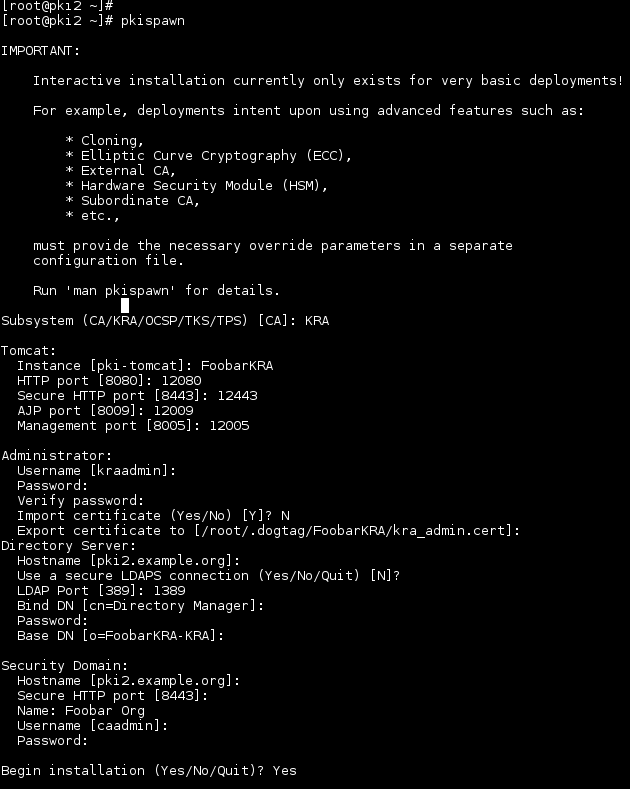
\includegraphics[width=80mm]{pkispawn-kra.png}
            \caption{pkispawn KRA subsystem}
        \end{figure}
\end{itemize}
\subsubsection{Installation Layout}
\begin{itemize}
    \item \textbf{/var/lib/pki/$<$instance$>$}: $<$Instance$>$ here is the tomcat Instance name 
        given during configuring subsystem
    \item \textbf{/var/lib/pki/$<$instance$>$/alias}: Is the NSS Database of the system where the subsystem system 
        certs are stored. When a subsystem is configured, Certain certificates are created for certain tasks 
        like Transport Cert for securely transporting private keys, storage cert for storing the private key, 
        These system certificates reside in alias directory. List of system certs are mentioned below, 
        All the below system certs are issued by CA during configuration of KRA.
        \begin{itemize}
            \item transportCert
            \item Server-Cert
            \item auditSigningCert
            \item storageCert
            \item subsystemCert
        \end{itemize}
    \item \textbf{/var/lib/pki/$<$instance$>$/conf/}: Configuration directory containing tomcat configuration,
        password file containing internal database(ldap) password, and NSS Database password
    \item \textbf{/var/lib/pki/$<$instance$>$/kra/}: Contains KRA Subsystem configuration file CS.cfg. This file is
        the main configuration file for KRA subsystem
    \item \textbf{/var/lib/pki/$<$instance$>$/lib/}: Contains kra subsystem related jar files 
    \item \textbf{/var/lib/pki/$<$instance$>$/bin/}: Tomcat related jar files
\end{itemize}
\subsubsection{Key Features}
\begin{itemize}
    \item Key Recovery Authority when configured with with certificate Manager(CA) stores private keys as part of
        certificate issuance process
    \item Supports two key recovery modes:
        \begin{itemize}
            \item Synchronous Recovery(Deprecated)
            \item Asynchronous Recovery
        \end{itemize}
    \item Supports Archiving passwords, symmetric keys, aka acts as a vault to store anything that needs
        to be stored securely and transported back securely
    \item Private keys are generally wrapped with a key called storage key and private keys
        while transporting are wrapped with transport keys, These keys can be rotated
\end{itemize}
\subsubsection{Architecture}
\begin{figure}[H]
    \centering
    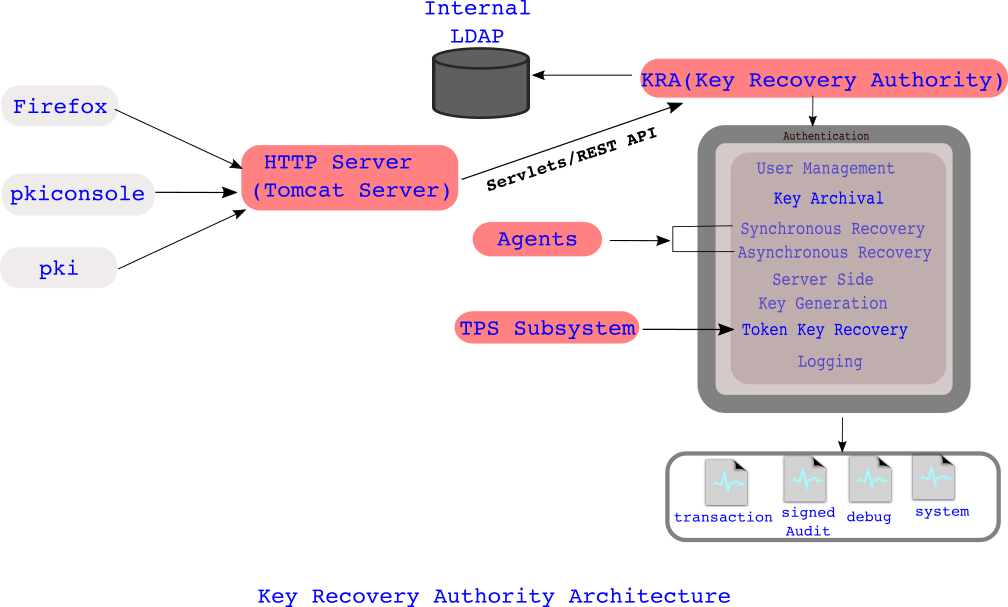
\includegraphics[width=80mm]{KRA-Architecture.png}
    \caption{KRA Architecture}
\end{figure}
\subsubsection{Interfaces}
\begin{itemize}
    \item End User Interface through \textbf{pki} cli
    \item Agent Interface(Browser/CLI)
    \item Admin Interface(Java console)
\end{itemize}
\subsubsection{Features}
\begin{itemize}
    \item Key Archival
        \begin{itemize}
            \item key archival is triggered when a user creates a certificate request through
                firefox(31.0 or older only)/pki/CRMFPopClient utility
            \item The key pair generated as part of the request(public/Private key) is submitted
                through a defined profile. 
            \item While submitting the private key is wrapped(encrypted) with transport cert(public key)
                and submitted to CA
            \item CA inturn retrieves the encrypted private key, decripts with transport private key 
            \item Private key is then stored in interan ldap of kRA by encrypting again with Storage Cert
            \item CA upon successful archival issues certificate
        \end{itemize}
        \begin{figure}[H]
            \centering
            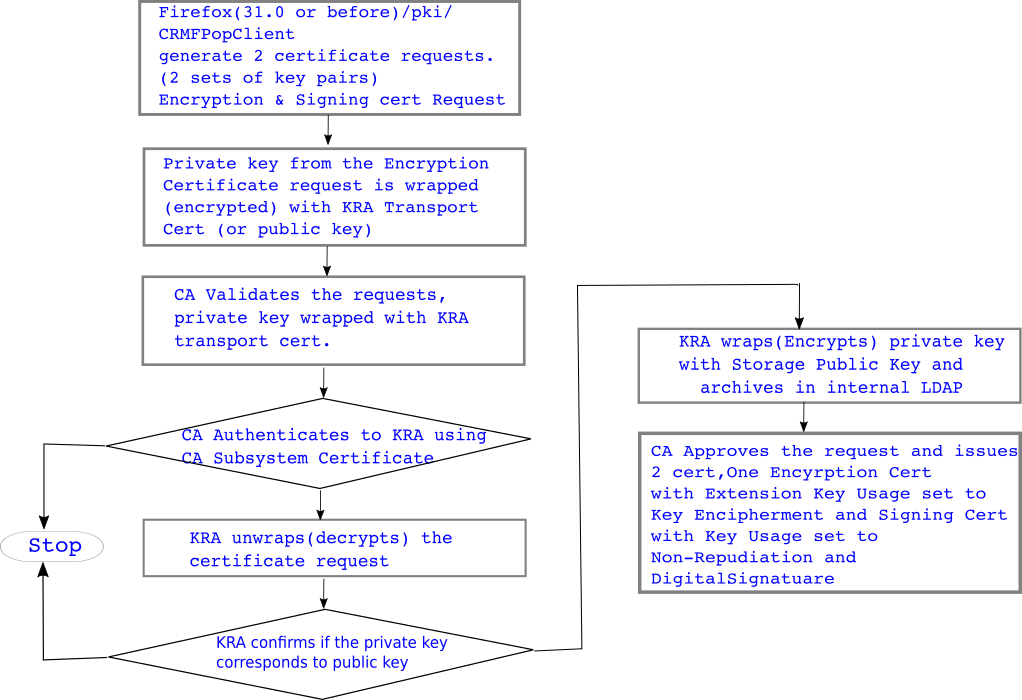
\includegraphics[width=100mm]{key-archival1.png}
            \caption{Key Archival Workflow}
        \end{figure}
        \begin{figure}[H]
            \centering
            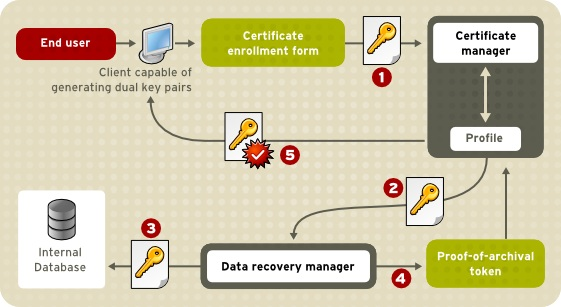
\includegraphics[width=70mm]{key-archival-process.png}
            \caption{Key Archival Process}
        \end{figure}
    \item Key Recovery
        \begin{itemize}
            \item KRA supports Agent initiated key recovery
            \item Designated Agents use the key recovery form on Agent services page
                to Approve/Reject key recovery
            \item CS uses m-of-n ACL-based recovery scheme
            \item CS uses it's ACL to ensure recovery agents are appropriately authenticated
                over SSL
            \item ACL also requires that agents belong to specific recovery agent group
            \item Recovery request is executed only when m of n agents have granted authorization
            \begin{figure}[H]
                \centering
                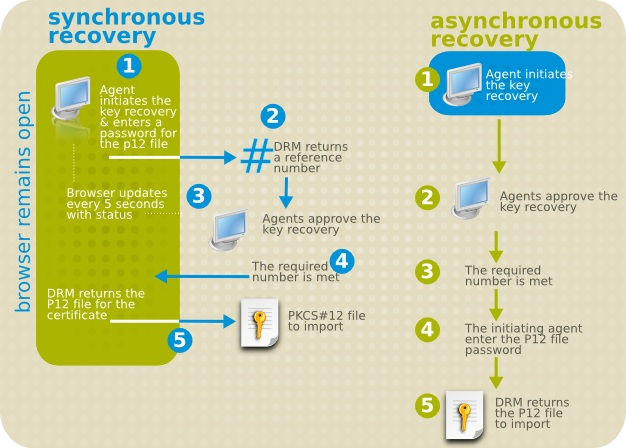
\includegraphics[width=70mm]{key-recovery.png}
                \caption{Key Recovery Process}
            \end{figure}
        \end{itemize}
    \item Archive Symmetric Keys, passwords, Asymetric keys (Vault)
        \begin{itemize}
            \item KRA has new REST interface to archive and recover 
                \begin{itemize}
                    \item Symmetric Keys
                    \item Random Security Data
                    \item Asymmetric Keys
                \end{itemize}
            \item This features is implemented through pki key CLI to generate, archive,retrieve
                keys.
        \end{itemize}
    \item Transport Key Rotation
        \begin{itemize}
            \item Transport Certs are created when KRA instance is configured using pkispawn
            \item Transport Certs are issued by CA to KRA
            \item Transport Certs public key is used to \textit{encrypt} private key while it's being
                transport by CA to KRA 
            \item In Large organizations, this transport key needs to be rotated. 
            \item The feature here adds support for second Transport Key 
        \end{itemize}
\end{itemize}
\subsubsection{Exercises}
    \begin{enumerate}[label*=\arabic*.]
        \item Setup required for KRA is same as CA, Refer \ref{setup1}, \ref{setup2}, \ref{setup3}, \ref{setup4}
        \item Setup KRA using pkispawn in separate Tomcat Instance. Use the below configuration with pkispawn
            \begin{enumerate}[label*=\arabic*.]
                \item Configure CA subsystem using method specified in \ref{rootca}
                \item Setup Directory Server for KRA subsystem  using below configuration
                    \begin{lstlisting}
[General]
FullMachineName=pki1.example.org
SuiteSpotUserID=nobody
SuiteSpotGroup=nobody

[slapd]
ServerIdentifier=Example1-RootKRA
ServerPort=1901
Suffix=dc=example,dc=org
RootDN=cn=Directory Manager
RootDNPwd=Secret123

[admin]
ServerAdminID=admin
ServerAdminPwd=Secret123
SysUser=nobody
                    \end{lstlisting}
                    \begin{lstlisting}[style=bashInputStyle]
$ setup-ds.pl --silent --file=kra-ds.inf --debug            
                    \end{lstlisting}
                \item \label{kra_sep_tomcat} Setup KRA using pkispawn in separate Tomcat Instance. Use the below configuration with pkispawn
                    \begin{lstlisting}
kra_inst.inf:

[DEFAULT]
pki_instance_name=Example1-RootKRA
pki_https_port=14443
pki_http_port=14080

#NSS DB Token Password
pki_token_password=Secret123

#RootKRA Admin password
pki_admin_password=Secret123

#Security Domain
pki_hostname=pki2.example.org
pki_security_domain_hostname=pki1.example.org
pki_security_domain_https_port=8443
pki_security_domain_user=caadmin
pki_security_domain_password=Secret123

#Client Dir
pki_client_dir=/opt/Example1-RootKRA
pki_client_pkcs12_password=Secret123
pki_client_database_password=Secret123

#Backup
pki_backup_keys=True
pki_backup_password=Secret123


[Tomcat]
pki_ajp_port=14009
pki_tomcat_server_port=14005

[KRA]
pki_admin_nickname=PKI KRA Administrator for Example Org
pki_import_admin_cert=False
pki_ds_hostname=pki1.example.org
pki_ds_ldap_port=1901
pki_ds_bind_dn=cn=Directory Manager
pki_ds_password=Secret123
                \end{lstlisting}
                \begin{lstlisting}[style=bashInputStyle]
$ pkispawn -s KRA -f kra_inst -vv            
                \end{lstlisting}
            \end{enumerate}
        \item \label{arch_privatekey} Enroll a certificate for user Foo1 and archive Private Key in KRA instance
            \begin{enumerate}[label*=\arabic*.]
                \item Create a NSS Database and Import CA Admin cert , CA cert. Refer:\ref{pki1}, \ref{pki2}, \ref{pki3}
                \item Import KRA Admin cert from /opt/Example1-RootKRA
                    \begin{lstlisting}[style=bashInputStyle]
$ pki -d /opt/rhqa_pki -c ’Secret123’ \
    client-cert-import --pkcs12 \
    /opt/Example1-RootKRA \
    --pkcs12-password Secret123
                    \end{lstlisting}
                    \begin{lstlisting}
Certificate Nickname                                         Trust Attributes
                                                             SSL,S/MIME,JAR/XPI

PKI Administrator for example.org                            u,u,u
Root CA                                                      CT,c,
PKI KRA Administrator for Example Org                        u,u,u                    
                    \end{lstlisting}
                \item Get the transportCert of the KRA instance 
                    \begin{lstlisting}[style=bashInputStyle]
$ certutil -L -d /var/lib/pki/Example1-RootKRA/alias/ \
    -n "transportCert cert-Example1-RootKRA KRA" \
    -a -o /opt/rhqa_pki/transportCert.pem                   
                    \end{lstlisting}
                \item Create a certificate request for user Foo1 to a profile in CA which archives private key
                    \begin{lstlisting}[style=bashInputStyle]
$ pki -d /opt/rhqa_pki -c 'Secret123' \
    -h pki1.example.org -p 8080 client-cert-request \
    "uid=foo1,O=Example Org" --profile caDualCert \
    --type crmf --transport transportCert.pem                    
                    \end{lstlisting}
                \item Approve The certificate request using CA Admin cert
                    \begin{lstlisting}[style=bashInputStyle]
$ pki -d /opt/rhqa_pki -c 'Secret123' \
    -h pki2.example.org -p 8080 \
    -n "PKI Administrator for example.org" \
    cert-request-review <request_id> --action approve                    
                    \end{lstlisting}
                \item Check Audit logs of KRA instance and see if the Archival request was successful
                \item Use kra key cli to list the keys archived
                    \begin{lstlisting}[style=bashInputStyle]
$ pki -d /opt/rhqa_pki -c 'Secret123' \
    -h pki1.example.org -p 14080 \
    -n "PKI KRA Administrator for Example Org" kra-key-find
                    \end{lstlisting}
            \end{enumerate}
        \item Archive Symmetric keys and passwords in Key Recovery Authority
            \begin{enumerate}[label*=\arabic*.]
                \item Setup: Create few role users in KRA subsystem and archive using different users instead of admin
                    \begin{enumerate}[label*=\arabic*.]
                        \item List all the Groups available for KRA Subsystem
                            \begin{lstlisting}[style=bashInputStyle]
$ pki -d /opt/rhqa_pki -c 'Secret123' -h pki1.example.org \
    -p 14080 -n "PKI KRA Administrator for Example Org" \
    kra-group-find                                
                            \end{lstlisting}
                        \item Create a User "KRA\_AgentV" and add him as member of \textbf{Data Recovery Manager Agents} 
                            \begin{lstlisting}[style=bashInputStyle]
$ pki -d /opt/rhqa_pki -c 'Secret123' \
-h pki1.example.org -p 14080 \
-n "PKI KRA Administrator for Exmaple Org" \
kra-user-add KRA_AgentV --fullName "KRA Agent User" \
--password 'Secret123'
-----------------------
Added user "KRA_AgentV"
-----------------------
  User ID: KRA_AgentV
  Full name: KRA Agent User
                            \end{lstlisting}
                        \item Create a Cert request for "KRA Agent User" using CA Subsystem 
                            \begin{lstlisting}[style=bashInputStyle]
#This command returns a request id , use the request id to approve the request
$ pki -d /opt/rhqa_pki -c 'Secret123' \
    -h pki1.example.org -p 8080 client-cert-request \
    "UID=KRA_AgentV,E=KRA_AgentV@example.org,CN="KRA Agent User",O=Example Org" 
                            \end{lstlisting}
                        \item Approve the certificate request using CA Admin User
                            \begin{lstlisting}[style=bashInputStyle]
#This command after approving the request returns certificate serial Number
$ pki -d  /opt/rhqa_pki -c 'Secret123' \
    -h pki1.example.org -p 8080 \
    -n "PKI Administrator for example.org" \
    cert-request-review <request_id> --action approve
-------------------------------
Approved certificate request 29
-------------------------------
 Request ID: 29
 Type: enrollment
 Request Status: complete
 Operation Result: success
 Certificate ID: 0x1d
                            \end{lstlisting}
                        \item Add the certificate created above to KRA Agent User
                            \begin{lstlisting}[style=bashInputStyle]
#This will prompt for the CA URL, specify CA's Non secure url(8080)                            
$ pki -d /opt/rhqa_pki -c 'Secret123' \
    -h pki1.example.org -p 14080 \
    -n "PKI KRA Administrator for Example Org" \
    kra-user-cert-add KRA_AgentV --serial \
    <certificate_serial_Number>
                            \end{lstlisting}
                        \item Make the KRA Agent user member of \textbf{"Data Recovery Manager Agents"}
                            \begin{lstlisting}[style=bashInputStyle]
$ pki -d /opt/rhqa_pki -c 'Secret123' \
    -h pki1.example.org -p 14080 \
    -n "PKI KRA Administrator for Example Org" \
    kra-group-member-add "Data Recovery Manager Agents" \
    KRA_AgentV
                            \end{lstlisting}
                        \item Import the KRA Agent Cert to NSS DB /opt/rhqa\_pki Directory
                            \begin{lstlisting}[style=bashInputStyle]
$  pki -d /opt/rhqa_pki -c 'Secret123'\
    -h pki1.example.org -p 8080 \
    client-cert-import "KRA_AgentV" \
    --serial \
    <certificate_serial_Number_of Agent_Cert>
                            \end{lstlisting}
                    \end{enumerate}
                \item \label{arch_password}  Archive a passphrase(password) using Agent User
                    \begin{lstlisting}[style=bashInputStyle]
$ pki -d /opt/rhqa_pki -c 'Secret123' \
    -h pki1.example.org -p 14080 \
    -n "KRA_AgentV" kra-key-archive \
    --clientKeyID beaker_server1 \
    --passphrase "MySecretSauce"
------------------------
Archival request details
------------------------
  Request ID: 0x2
  Key ID: 0x2
  Type: securityDataEnrollment
  Status: complete
                    \end{lstlisting}
                \item \label{arch_symmetric} Generate Symmetric keys with AES algo of size 128 and archive it
                    \begin{lstlisting}[style=bashInputStyle]
$ pki -d /opt/rhqa_pki -c 'Secret123' \
    -h pki1.example.org -p 14080 \
    -n "KRA_AgentV" kra-key-generate \
    --key-algo aes --key-size 128 \
    --usages wrap 
                    \end{lstlisting}
            \end{enumerate}
        \item  Retrieve archived symmetric/Asymmetric keys 
            \begin{enumerate}[label*=\arabic*.]
                \item Retrieve Archived Symmetric key using \textbf{key-retreive}
                    \begin{lstlisting}[style=bashInputStyle]
$ pki -d /opt/rhqa_pki -c 'Secret123' \
    -h pki1.example.org -p 14080 \
    -n "KRA_AgentV" kra-key-retrieve --keyID <KEY_ID>
                    \end{lstlisting}
                \item Retrieve Archived Passwords , Refer \ref{arch_password}
                    \begin{lstlisting}[style=bashInputStyle]
$ pki -d /opt/rhqa_pki -c 'Secret123' \
    -h pki1.example.org -p 14080 \
    -n "KRA_AgentV" kra-key-retrieve --keyID <KEY_ID>
                    \end{lstlisting}
                \item Retrieve Asymmetric keys (private Key). Refer Section \ref{arch_privatekey}
                    \begin{lstlisting}[style=bashInputStyle]
$ pki -d /opt/rhqa_pki -c 'Secret123' \
    -h pki1.example.org -p 14080 \
    -n "KRA_AgentV" kra-key-retrieve --keyID <KEY_ID>
                    \end{lstlisting}
                \item Retrieving Asymmetric Keys From Browser(firefox)
                    \begin{itemize}
                        \item Import CA Admin Cert and KRA Admin p12 file to Firefox browser
                        \item Trust the CA cert 
                        \item Access KRA Agent Page \textit{https://pki1.example.org:14443}
                        \item Authenticate it with KRA Agent Cert
                        \item Click "Recover Keys" 
                        \item From the Available Recovery Options select "Certificate"
                        \item Paste the Certificate foo1 user archived, use CA EE interface to get the certificate
                        \item Click on Show key 
                        \item From the Search Results , Click on "Recover"
                        \item In the Next screen , Select "Async Recovery", Click on "Recover"
                        \item This should return a Key Recovery Status with reference Number
                        \item Click on The request Number and "Grant" the request
                        \item click on the request id shown on the page
                        \item Specify the PKCS12 Password and click on Retrieve PKCS12
                    \end{itemize}
            \end{enumerate}
        \item Transport Key Rotation
            \begin{enumerate}[label*=\arabic*.]
                \item Setup CA clone , Refer to steps described in Section: \ref{clone_rootca}
                \item Setup KRA Clone
                    \begin{enumerate}[label*=\arabic*.]
                        \item While setting up KRA instance (Refer Section: \ref{kra_sep_tomcat}, we had
                            backed the system keys using parameter \texttt{pki\_backup\_keys=True}. This 
                            is equivalent of PKCS12Export ran in section \ref{pkcs12export} 
                        \item The backup of system keys of KRA is saved in alias Directory of KRA which is
                            \texttt{/var/lib/pki/Example1-RootKRA/alias/}
                            \begin{lstlisting}[style=bashInputStyle]
# ls -l /var/lib/pki/Example1-RootKRA/alias/
total 104
-rw-------. 1 pkiuser pkiuser 65536 Jan 31 17:17 cert8.db
-rw-------. 1 pkiuser pkiuser 28672 Feb  1 17:08 key3.db
-rw-r--r--. 1 pkiuser pkiuser 11327 Jan 31 17:17 kra_backup_keys.p12
-rw-------. 1 pkiuser pkiuser 16384 Jan 31 17:16 secmod.db
                            \end{lstlisting}
                        \item Copy the kra\_backup\_keys.p12 to clone system \texttt{pki2.example.org}

                        \item Setup Directory server on clone system for KRA
                            \begin{lstlisting}
[General]
FullMachineName=pki2.example.org
SuiteSpotUserID=nobody
SuiteSpotGroup=nobody

[slapd]
ServerIdentifier=Foobar1-CloneKRA
ServerPort=1902
Suffix=dc=example,dc=org
RootDN=cn=Directory Manager
RootDNPwd=Secret123

[admin]
ServerAdminID=admin
ServerAdminPwd=Secret123
SysUser=nobody
                            \end{lstlisting}
                        \item Setup Clone KRA using below configuration
                            \begin{lstlisting}
clone_kra.inf :

[DEFAULT]
pki_instance_name=Example1-CloneKRA
pki_https_port=14443
pki_http_port=14080

# Token password
pki_token_password=Secret123

#Security Domain
pki_security_domain_hostname=pki1.example.org
pki_security_domain_https_port=8443
pki_security_domain_user=caadmin
pki_security_domain_password=Secret123

# Admin Password
pki_admin_password=Secret123

# client Dir
pki_client_pkcs12_password=Secret123
pki_client_database_password=Secret123
pki_client_dir=/opt/Example1-CloneKRA


[Tomcat]
pki_ajp_port=14009
pki_tomcat_server_port=14005

[KRA]
pki_clone=True
pki_clone_pkcs12_password=Secret123
pki_clone_pkcs12_path=/tmp/kra_backup_keys.p12
pki_clone_replication_master_port=1901
pki_clone_replication_clone_port=1902
pki_clone_repicate_schema=True
pki_clone_uri=https://pki1.example.org:14443
pki_import_admin_cert=False
pki_ds_hostname=pki3.example.org
pki_ds_ldap_port=1902
pki_ds_bind_dn=cn=Directory Manager
pki_ds_password=Secret123
pki_ds_secure_connection=False
pki_ds_remove_data=True
pki_ds_base_dn=o=Example1-RootKRA-KRA
                            \end{lstlisting}
                            \begin{lstlisting}[style=bashInputStyle]
$ pkispawn -s KRA -f clone_kra.inf -vv                            
                            \end{lstlisting}
                        \item Request a new DRM Transport Cert
                            \begin{enumerate}[label*=\arabic*.]
                                \item Stop the Master KRA instance 
                                    \begin{lstlisting}
$ systemctl stop pki-tomcatd@Example1-RootKRA                                    
                                    \end{lstlisting}
                                \item Go to KRA's NSS DB directory and take the backup of existing NSS DB in a subdirectory
                                    called backup
                                    \begin{lstlisting}[style=bashInputStyle]
$ cd /var/lib/pki/Example1-RootKRA/kra/alias
$ mkdir backup
$ cp -a *.db backup             
                                    \end{lstlisting}
                                \item \label{transport-new-pkcs10} Create a new pkcs10 request
                                    \begin{lstlisting}[style=bashInputStyle]
$  PKCS10Client -p <password> -d '.' -o 'req.txt' -n 'CN=DRM Transport 2 Certificate,O=Example Org'
                                    \end{lstlisting}
                                    \textbf{Note:} password of NSS Database can be found in password.conf in conf directory of KRA instance
                                \item Submit the certificate request to CA using EE interface and approve the request using Agent inteface
                                    \begin{itemize}
                                        \item Open the CA EE Page and select profile "Manual Data recovery Manager transport certificate Enrollment"
                                        \item paste the certificate request created in step \ref{transport-new-pkcs10}  and submit the request
                                        \item From CA Agent page approve the request
                                    \end{itemize}
                                \item Get the approved cert  and save the base64 format in a file new-drm-transport.pem
                                \item Import the DRM Certificate in NSSDB and Update DRM Configuration
                                    \begin{lstlisting}[style=bashInputStyle]
$ certutil -d /var/lib/pki/Example1-RootKRA/alias \
    -A -n "transportCert-new Cert-Example1-Rootkra KRA" \
    -t u,u,u -i new-drm-transport.pem 
                                    \end{lstlisting}
                                \item Add the new transport certs nick name in KRA's CS.cfg
                                    \begin{lstlisting}
kra.transportUnit.newNickName=transportCert-new Cert-Example1-Rootkra KRA
                                    \end{lstlisting}
                                \item Update the CA's CS.cfg with new transport Certificate
                                    \begin{lstlisting}[style=bashInputStyle]
$cp new-drm-transport.pem new-drm-transport-backup.pem                                    

$ unix2dos new-drm-transport-backup.pem
# remove cetificate headers 
$ cat new-drm-transport.pem | perl -p -i -e 's/\r\n//'
                                    \end{lstlisting}
                                    
                                    Copy the output of above command and edit CA CS.cfg and replace the exisiting transport Cert

                                    \begin{lstlisting}
ca.connector.KRA.transportCert=<new transport cert> [ base64 cert which has been trimmed in to one line]                                    
                                    \end{lstlisting}

                                \item Restart CA and KRA instances
                                \item Perform Archival Operation as specified in section: \ref{arch_privatekey} with new transport cert
                            \end{enumerate}
                    \end{enumerate}
            \end{enumerate}
    \end{enumerate}
\subsection{Online Certificate Status Protocol}
\subsubsection{Introduction}
    \begin{itemize}
        \item Online Certificate Status Manager is an subsystem external to CA.
        \item This subsystem acts as an external OCSP which can be publicly accessible.
        \item Multiple CA's can publish CRL to a single OCSP 
        \item Clients can verify certs using OCSP 
    \end{itemize}
\subsubsection{Installation}
    \begin{itemize}
        \item RPM: \textbf{pki-ocsp}
            OCSP subsystem can be configured through pkispawn using interactive or to have a customize
            setup a separate file can be specified with pkispawn

            OCSP subsystem can share the same tomcat instance created by the CA subsystem which allows
            OCSP to use same ports as that of CA.
            \begin{figure}[H]
                \centering
                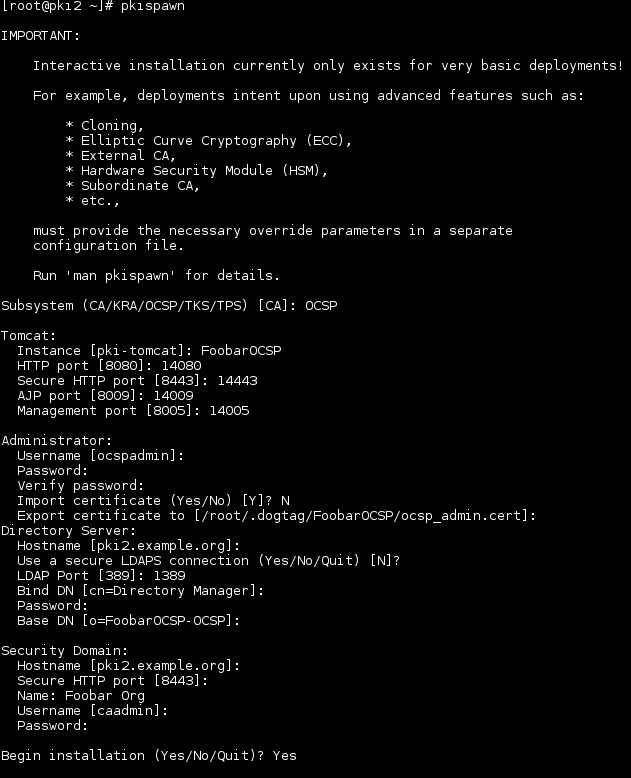
\includegraphics[width=80mm]{pkispawn-ocsp.png}
                \caption{pkispawn KRA subsystem}
            \end{figure}
    \end{itemize}
\subsubsection{Interfaces}
\begin{itemize}
    \item End User Interface through \textbf{pki} cli
    \item Agent Interface(Browser/CLI)
    \item Admin Interface(Java console)
\end{itemize}
\subsubsection{Exercises}
\subsection{SmartCard Management}
\subsubsection{Introduction}
    \begin{itemize}
        \item \textbf{What:} Smartcard contains an embedded microprocessor. This microprocess runs Java Virtual Machine(JVM) and 
            provides environment to run applications on top of it. 
            \begin{itemize}
                \item Smartcard contains a chip with java on it. 
                \item it contains a JVM, Java Runtime Environment, and some API for applications to access the card.
            \end{itemize}
        \item \textbf{Why:} 
            \begin{itemize}
                \item Smartcards are typically used by enterprise to provide identification and authentication
                \item Smartcards provide 2-Factor Authentication which is 
                    \begin{itemize}
                        \item Something you have - smartcard
                        \item Something you know - pin(password) to access the smartcard
                    \end{itemize}
            \end{itemize}
        \item \textbf{Use cases:}
            \begin{itemize}
                \item System Authentication using Smartcard (Linux/Windows System Authentication)
                \item Secure VPN Access
                \item Email Signature and Encryption
                \item Disc Encryption
            \end{itemize}
        \item \textbf{How:}
            \begin{itemize}
                \item For enterprise to use smartcard a digital Certificate is issued to the smartcard
                \item This certificate is used to identify the user of the smartcard
                \item User uses digital certificate on the smartcard to perform 2-factor authentication 
            \end{itemize}
        \item \textbf{Mangement:}
            \begin{itemize}
                \item We need a management software to manage certificates on the smartcard
                    \begin{itemize}
                        \item Enrolling certificate
                        \item Formatting Smartcard
                        \item What to do with the certificate if smartcard is lost
                        \item What to do if the user of the smartcard is no longer in the company
                    \end{itemize}
                \item To do the above operations, we have Token Management system in Certificate Services which comprises of the following:
                    \begin{itemize}
                        \item \textbf{TPS}: The Token Processing System (TPS) interacts with smart cards to help them generate and store
                            keys and certificates for a specific entity, such as a user or device.
                        \item \textbf{TKS}: The Token Key Service (TKS) generates, or derives, symmetric keys used for communication
                            between the TPS and smart card.
                        \item \textbf{CA}: The Certificate Authority (CA) creates and revokes user certificates stored on the smart card.
                        \item \textbf{KRA}: Optionally, the Key Recovery Authority (KRA) archives and recovers keys for the smart card.
                        \item \textbf{Enterprise Security Client}: is the conduit through which TPS communicates with each token over
                            a secure HTTP channel (HTTPS), and, through the TPS, with the Certificate System.
                    \end{itemize}
            \end{itemize}
    \end{itemize}
\subsubsection{Architecture}
\begin{figure}[H]
    \centering
    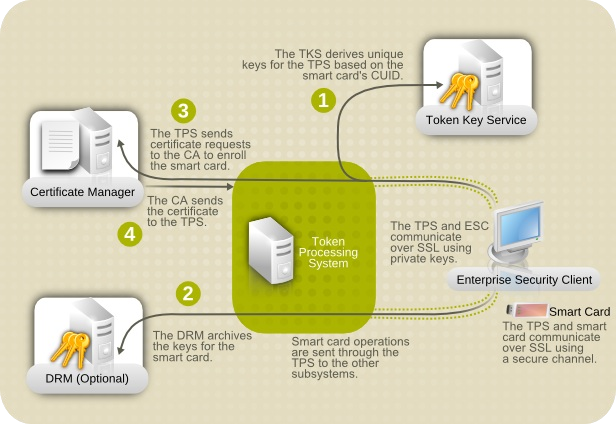
\includegraphics[width=80mm]{TMS-workflow.png}
    \caption{Token Management System}
\end{figure}
\subsubsection{Common Terms Used with regard to Smartcard}
    \begin{itemize}
        \item Secure Channel Protocol: A secure communication protocol and set of security protocol used to 
            create a secure channel with token during TPS Operations.
        \item Applets: TPS communicates with an applet on the smartcard. 
        \item APDU(Application Protocol Data Unit): Standard communication messaging protocol between a card accepting device(Reader)
            and a smart card 
        \item SmartCards come with a cardmanager applet and a vendor applet or with only card manager applet. 
        \item Coolkey: applet is the supported Card Manager applet
        \item Smartcard has cryptographic functionality supporting symmetric and Assymetric Encryption(like RSA)
        \item CCID: CCID (chip card interface device) protocol is a USB protocol that allows a smartcard to be 
            connected to a computer via a card reader using a standard USB interface, without the need for 
            each manufacturer of smartcards to provide its own reader or protocol.~\cite{wiki:ccid}
    \end{itemize}
\subsubsection{Token Key Service}
    \begin{itemize}
        \item Introduction
            \begin{itemize}
                \item A subsystem in the token management system which derives specific, separate keys for every
                    smart card based on the smart card APDUs and other shared information, like the token CUID.~\cite{RedHat:AdminGuide}
                \item The TKS derives keys based on the token CCID, private information, and a defined algorithm. 
                    These derived keys are used by the TPS to format tokens and enroll, or process, certificates on the token(smartcard).~\cite{RedHat:AdminGuide}
                \item TKS and TPS have a sharedSecret to wrap sensitive info sent between TKS and TPS
            \end{itemize}
        \item Features:
            \begin{itemize}
                \item \textbf{Manage shared keys}
                    \begin{itemize}
                        \item Token Key Service (TKS) derives keys for the TPS to use.
                        \item Based on Token CUID, and other token material , Derive keys that encrypt session between TPS and ESC
                        \item Keys are derived based on Common Master Key which is known to TKS and existent on smartcards
                    \end{itemize}
                \item \textbf{Generate Master Key}
                    \begin{itemize}
                        \item Master key is 3DES symmetric Key stored in software/Hardware
                        \item Transport Key wraps the other keys derived(from master key) and used by TKS and TPS
                    \end{itemize}
            \end{itemize}
    \end{itemize}
\subsubsection{Token Processing Service}
    \begin{itemize}
            \item Introduction
                \begin{itemize}
                    \item TPS interacts with smart cards to help them generate and store keys and certificates for a specific entity
                    \item Smart card operations go through TPS and are forwarded to the appropriate subsystem for action, 
                        such as the Certificate Authority to generate certificates or the Key Recovery Authority to archive and recover key
                \end{itemize}
            \item Features
                \begin{itemize}
                    \item Secure Channel
                        \begin{itemize}
                            \item The Token Key Service (TKS) generates the (token) keys (a set of 3 keys derived) from Master keys
                            \item These keys are used by TPS to communicate with ESC(smartcard)
                            \item TPS communicates with the TKS over SSL but TPS communicates with ESC over secure channel
                            \item Every smartcard has 3 keys:
                                \begin{itemize}
                                    \item An \textbf{auth key} which is used for encryption and authentication: a session key dervied from the auth key
                                        each time a secure channel is opened.
                                    \item A \textbf{MAC key} which is used for message authentication; like the auth keys, a session key is derived
                                        from the MAC key each time a secure channel is opened.
                                    \item A \textbf{key encryption key (KEK)} which is to encrypt the session keys.
                                \end{itemize}
                            \begin{figure}[H]
                                \centering
                                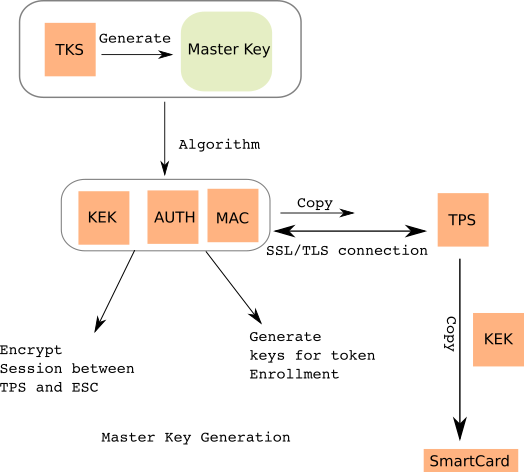
\includegraphics[width=80mm]{tks-key-derivation1.png}
                                \caption{TKS Key Derivation}
                            \end{figure}
                        \end{itemize}
                    \item Supported TPS Operations
                        \begin{itemize}
                            \item Formatting Smartcards
                            \item Resetting PIN on smartcards
                            \item Upgrading the applet for smartcard tokens
                            \item Perform LDAP Authentication
                            \item Managing token database
                            \item Logging Token events
                        \end{itemize}
                    \item Token Profiles
                        \begin{itemize}
                            \item Just like certificate profiles there are different token profiles to format different kind of tokens 
                            \item Token profiles define the below:
                                \begin{itemize}
                                    \item The steps to format and enroll the token
                                    \item The configuration of the final enrolled token
                                    \item Profiles also specify which LDAP server to be used for authentication and 
                                        which CA should be used for enrolling certificates
                                    \item List of Token profiles:
                                        \begin{figure}[H]
                                            \centering
                                            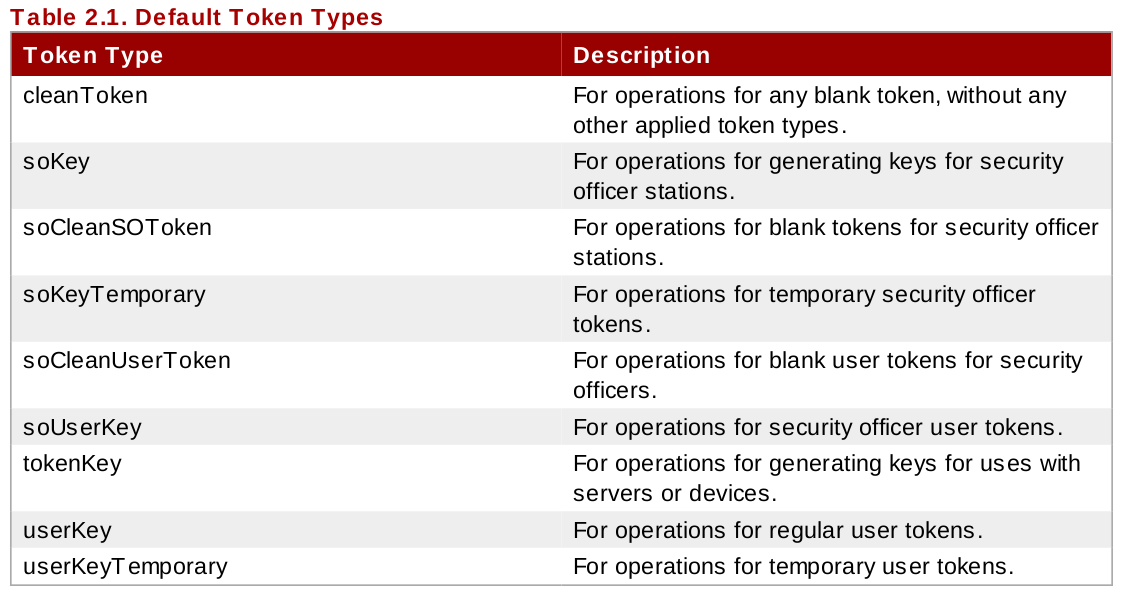
\includegraphics[width=80mm]{tokenprofiles1.png}
                                            \caption{List of Token Profiles}
                                        \end{figure}
                                \end{itemize}
                        \end{itemize}
                    \item TPS-TKS-Smartcard Workflow
                        \begin{figure}[H]
                            \centering
                            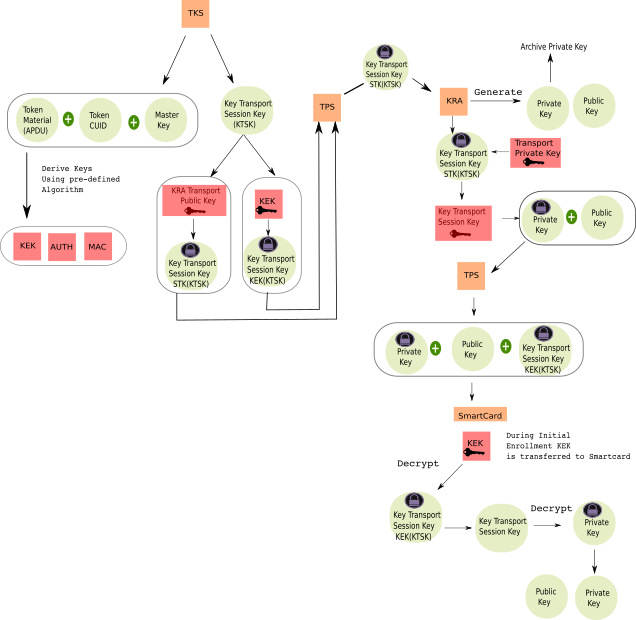
\includegraphics[width=120mm]{tks-tps-drm-esc-enrollment2.png}
                            \caption{TPS-TKS-Smartcard Worfklow}
                        \end{figure}
                    \item TKS Configuration 
                        \begin{itemize}
                            \item RPM: \textbf{pki-tks}
                            \item Configuration: TKS subsystem can be configured through pkispawn using interactive or to have a 
                                customize setup a separate file can be specified with pkispawn
                            \item TKS subsystem can share the same tomcat instance created by the CA subsystem which allows 
                                TKS to use same ports as that of CA
                            \begin{figure}[H]
                                \centering
                                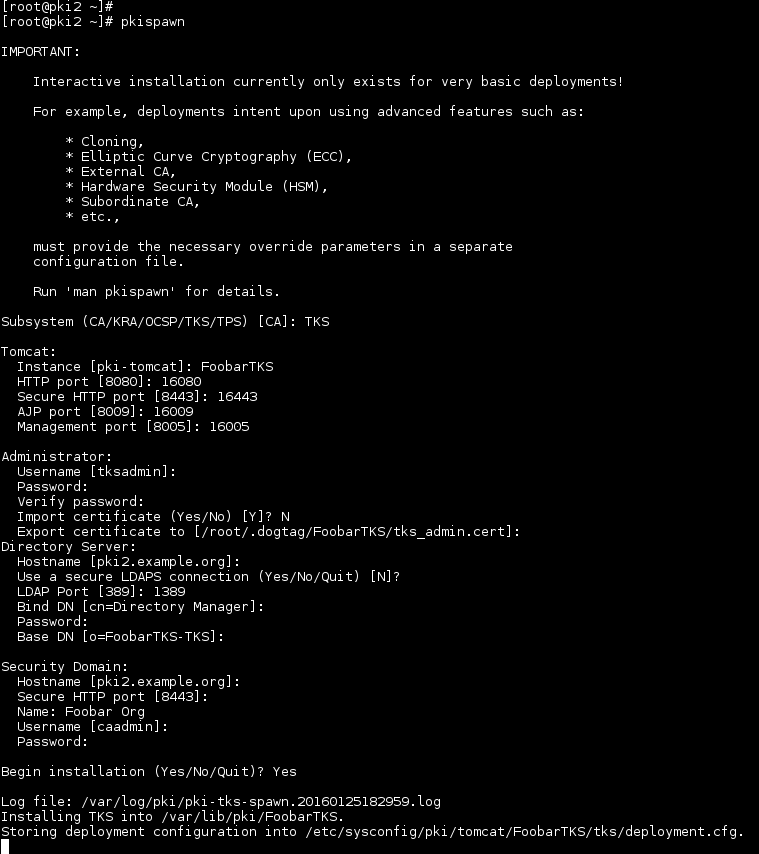
\includegraphics[width=80mm]{pkispawn-tks.png}
                                \caption{Interactive installation of TKS using pkispawn}
                            \end{figure}
                        \end{itemize}
                    \item Creating sharedSecret 
                        \begin{itemize}
                            \item TKS generates a \textbf{\underline{sharedSecret}} to wrap sensitive information passed over TPS.
                            \item This sharedSecret is to be created on TKS NSS database using tool called \textbf{tkstool}
                            \begin{figure}[H]
                                \centering
                                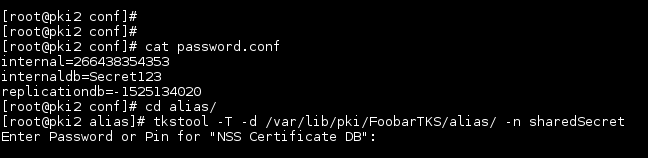
\includegraphics[width=50mm]{tkstool-create-sharedSecret1.png}
                                \caption{NSS Internal database password}
                            \end{figure}
                            \begin{figure}[H]
                                \centering
                                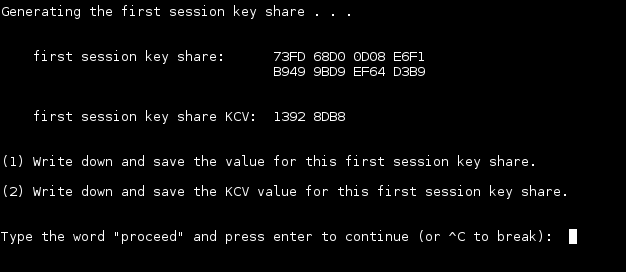
\includegraphics[width=50mm]{tkstool-create-sharedSecret2.png}
                                \caption{tkstool Usage}
                            \end{figure}
                            \begin{figure}[H]
                                \centering
                                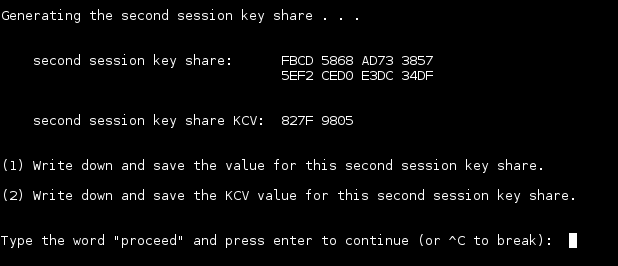
\includegraphics[width=50mm]{tkstool-create-sharedSecret3.png}
                                \caption{First Session Key}
                            \end{figure}
                            \begin{figure}[H]
                                \centering
                                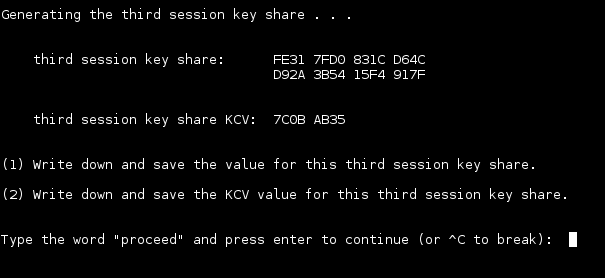
\includegraphics[width=50mm]{tkstool-create-sharedSecret4.png}
                                \caption{Second Session Key}
                            \end{figure}
                            \begin{figure}[H]
                                \centering
                                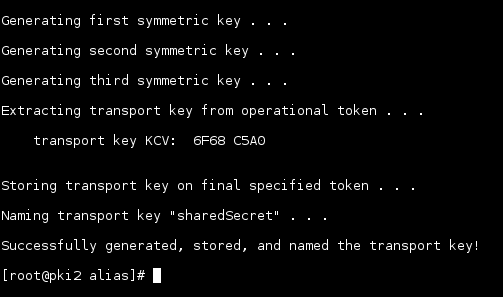
\includegraphics[width=50mm]{tkstool-create-sharedSecret5.png}
                                \caption{Third Session Key}
                            \end{figure}
                            \item tkstool utility prints out the key shares and KCV values for each of the three
                                session keys that are generated. These are necessary to import the \textbf{sharedSecret} to TPS
                        \end{itemize}
                    \item TPS Configuration
                        \begin{itemize}
                            \item RPM: \textbf{pki-tps}
                                \item Configuration: TPS subsystem can be configured through pkispawn using interactive or to have a
                                    customize setup a separate file can be specified with pkispawn
                                \item TPS subsystem can share the same tomcat instance created by the CA subsystem which allows
                                    TPS to use same ports as that of CA
                                \begin{figure}[H]
                                    \centering
                                    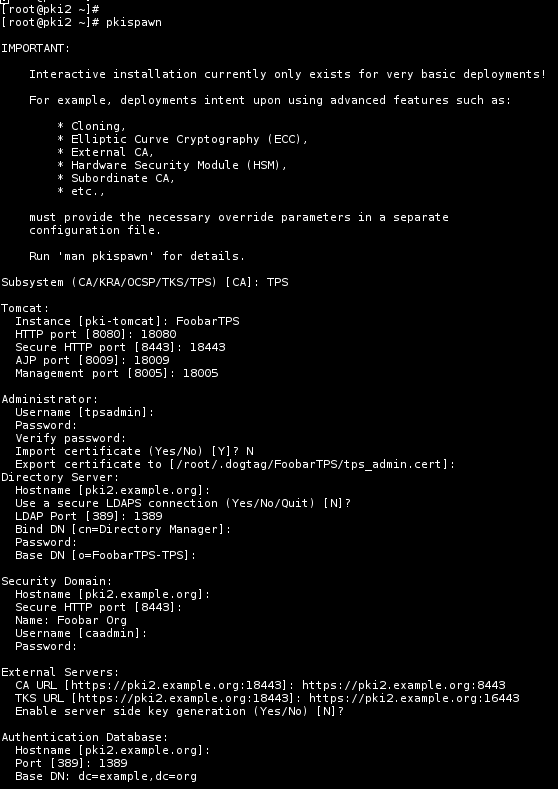
\includegraphics[width=80mm]{pkispawn-tps.png}
                                    \caption{Interactive installation of TKS using pkispawn}
                                \end{figure}
                                \begin{figure}[H]
                                    \centering
                                    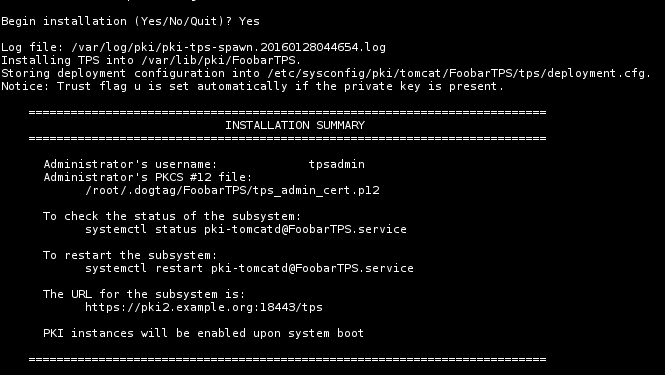
\includegraphics[width=80mm]{pkispawn-tps2.png}
                                    \caption{Continuation of pkispawn}
                                \end{figure}
                            \item Import SharedSecret
                                \begin{itemize}
                                    \item Import the sharedSecret created by TKS so that TKS and TPS can wrap sensitive information
                                    \item sharedSecret needs to be imported in to TPS NSS Database
                                \end{itemize}
                                \begin{figure}[H]
                                    \centering
                                    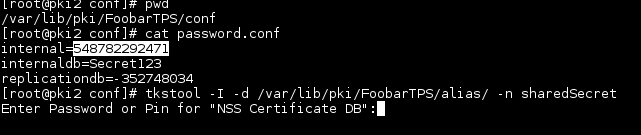
\includegraphics[width=80mm]{tkstool-import-sharedSecret1.png}
                                    \caption{Get NSS Password of TPS NSS database}
                                \end{figure}
                                \begin{figure}[H]
                                    \centering
                                    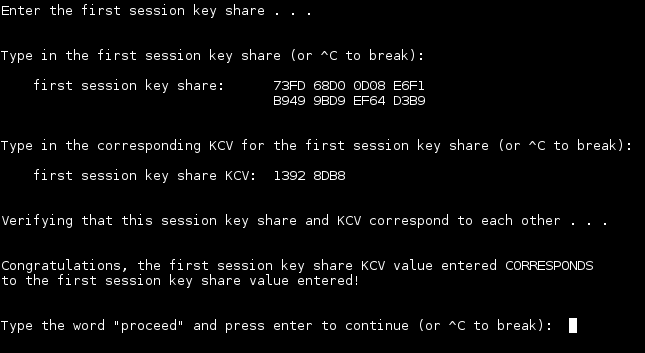
\includegraphics[width=80mm]{tkstool-import-sharedSecret2.png}
                                    \caption{tkstool to import first session key}
                                \end{figure}
                                \begin{figure}[H]
                                    \centering
                                    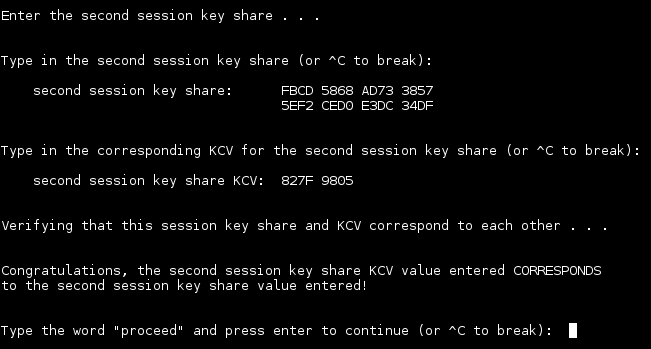
\includegraphics[width=80mm]{tkstool-import-sharedSecret4.png}
                                    \caption{tkstool to import second session key}
                                \end{figure}
                                \begin{figure}[H]
                                    \centering
                                    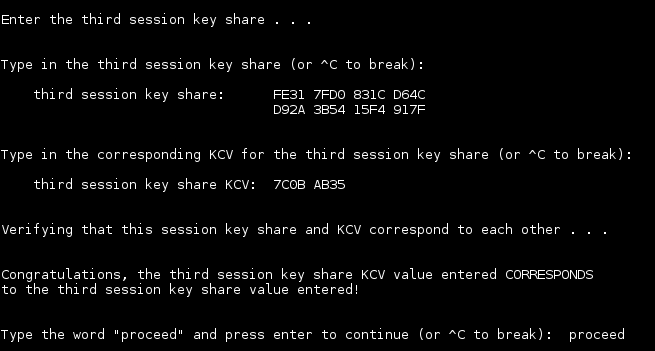
\includegraphics[width=80mm]{tkstool-import-sharedSecret5.png}
                                    \caption{tkstool to import third session key}
                                \end{figure}
                            \item TKS Instance Layout
                                \begin{itemize}
                                    \item 
                                \end{itemize}
                        \end{itemize}
                \end{itemize}
    \end{itemize}
\bibliography{references}
\end{document} 
